\documentclass[11pt,a4paper]{article}

\usepackage[margin=2.4cm]{geometry}
\usepackage[T1]{fontenc}
\usepackage[utf8]{inputenc}
\usepackage{lmodern}
\usepackage{microtype}
\usepackage{amsmath,amssymb,bm}
\usepackage{booktabs}
\usepackage{graphicx}
\usepackage{tabularx}
\usepackage{longtable}
\usepackage{pdflscape}
\usepackage{array}
\usepackage{xcolor}
\usepackage[numbers,sort&compress]{natbib}
\usepackage[hidelinks]{hyperref}
\usepackage{url}

\emergencystretch=3em
\newcolumntype{L}[1]{>{\raggedright\arraybackslash}p{#1}}
\newcommand{\X}{\mathbf{X}}
\newcommand{\Y}{\mathbf{Y}}
\newcommand{\A}{\mathbf{A}}
\newcommand{\K}{\mathbf{K}}
\newcommand{\B}{\mathbf{B}}
\newcommand{\Z}{\mathbf{Z}}
\newcommand{\T}{\mathbf{T}}
\newcommand{\transpose}{^{\mathsf T}}
\newcommand{\code}[1]{\nolinkurl{#1}}

\title{\textbf{Supplementary Material}\\
One-shot screening of linear preprocessing operators for PLS and Ridge calibration in near-infrared spectroscopy}

\author{
Gr{\'e}gory Beurier \quad Robin Reiter \quad Camille No{\^u}s\\[0.35em]
Lauriane Rouan \quad Denis Cornet
}

\date{Supplement of May 17, 2026}

\begin{document}
\maketitle

\tableofcontents

\section{Notation, Scope and Complete Derivations}

\subsection{Strict linear operators}

Let $\X\in\mathbb{R}^{n\times p}$ be a spectral matrix and
$\Y\in\mathbb{R}^{n\times q}$ a response matrix.  A strict linear spectral
operator $\A_b\in\mathbb{R}^{p\times p}$ acts on row spectra as
\begin{equation}
  \X_b=\X\A_b\transpose .
\end{equation}
The operator is fixed once the wavelength grid and hyperparameters are fixed.
The compact bank contains identity, Savitzky--Golay smoothers and
derivatives, finite differences and polynomial detrending projections.

Sample-adaptive or fitted transformations do not satisfy this definition.
SNV uses sample-specific statistics, MSC and EMSC estimate correction
parameters relative to a reference, and ASLS solves an asymmetric baseline
problem.  They are valid preprocessing branches, but they are fitted inside
each calibration fold and are not inserted into the strict-linear operator
identities.

\subsection{AOM-PLS covariance identity}

For centered $\X$ and $\Y$, standard PLS can be written with weights
$\mathbf W$, loadings $\mathbf P$ and response loadings $\mathbf Q$:
\begin{equation}
  \B=\mathbf W(\mathbf P\transpose\mathbf W)^+\mathbf Q\transpose .
\end{equation}
For a fixed operator $\A_b$,
\begin{equation}
  (\X\A_b\transpose)\transpose\Y
  =
  \A_b\X\transpose\Y .
  \label{eq:sup_cov_identity}
\end{equation}
Equation~\ref{eq:sup_cov_identity} is the algebraic reason why strict-linear
preprocessing alternatives can be evaluated in covariance space.  The
SIMPLS-covariance implementation acts on $\X\transpose\Y$ directly.  The
NIPALS-adjoint implementation applies $\A_b$ and $\A_b\transpose$ during the
iterative extraction without storing every transformed design matrix.

If a transformed-space direction for component $a$ is $r_a$, the
original-wavelength direction is
\begin{equation}
  z_a=\A_b\transpose r_a .
\end{equation}
With $\Z=[z_1,\ldots,z_k]$ and $\T=\X\Z$, the final coefficient matrix is
\begin{equation}
  \B=\Z(\mathbf P\transpose\Z)^+\mathbf Q\transpose .
  \label{eq:sup_aompls_coef}
\end{equation}
Thus the fitted AOM-PLS object predicts from original spectra and can expose
coefficients on the original wavelength grid.

\subsection{AOM-Ridge kernels}

For centered $\X_c$ and $\Y_c$, a single operator induces
\begin{align}
  \mathbf Z_b &= \X_c\A_b\transpose,\\
  \K_b &= \mathbf Z_b\mathbf Z_b\transpose
       = \X_c\A_b\transpose\A_b\X_c\transpose,\\
  \mathbf C_b &= (\K_b+\alpha\mathbf I_n)^{-1}\Y_c,
\end{align}
and the recovered original-space coefficient matrix is
\begin{equation}
  \bm\beta_b=\A_b\transpose\A_b\X_c\transpose\mathbf C_b .
\end{equation}
For weighted operator mixtures,
\begin{equation}
  \K=\sum_{b=1}^{m}s_b^2\X_c\A_b\transpose\A_b\X_c\transpose,
  \qquad
  \mathbf M=\sum_{b=1}^{m}s_b^2\A_b\transpose\A_b,
\end{equation}
so
\begin{equation}
  \bm\beta=\mathbf M\X_c\transpose(\K+\alpha\mathbf I_n)^{-1}\Y_c.
\end{equation}
This is the Ridge counterpart of AOM-PLS: PLS adapts supervised
cross-covariance directions, while Ridge adapts the regularized sample
geometry.

\subsection{Ridge selector family}

The main manuscript now reports both the plain global compact selector and the
Blender selector.  The full Ridge family also includes branch-specific compact
variants, local-neighbourhood selectors and multi-branch kernel mixtures.
Global selectors choose one operator geometry for the whole calibration set.
Local selectors restrict the geometry to neighbourhoods such as $k=50$ nearest
calibration samples.  Multi-branch kernels combine several branch geometries
with shrinkage.  These variants are useful for understanding the design space,
but their refreshed paired statistics do not beat Blender on the main Ridge
denominators.

\subsection{FastAOM derivation}

FastAOM is treated here as an exploration of alternative AOM forms, not as a
main result.  It defines a chain as an ordered composition of primitive
strict operators.  The grammar assigns roles to operators:
baseline/projection, smoothing, derivative and projection-mask operations.  A
depth cap limits the number of composed operators, and grammar pruning removes
invalid or redundant role sequences before screening.

For each fold-local base $B_j(\X)$ and chain $s$, FastAOM computes
\begin{equation}
  \mathrm{score}(j,s)
  =
  \frac{\left\|A_s B_j(\X_c)\transpose y_c\right\|_2^2}
       {\left\|B_j(\X_c)A_s\transpose\right\|_F^2
        \left\|y_c\right\|_2^2}.
\end{equation}
With a truncated SVD $B_j(\X_c)\approx U_j\Sigma_jV_j\transpose$ and
$F_{j,s}=A_sV_j\Sigma_j$, the screened kernel is approximated by
\begin{equation}
  \K_{j,s}
  =
  B_j(\X_c)A_s\transpose A_s B_j(\X_c)\transpose
  \approx U_j C_{j,s}U_j\transpose,
  \qquad
  C_{j,s}=F_{j,s}\transpose F_{j,s}.
\end{equation}

\begin{table}[h]
\centering
\caption{FastAOM model families.  These are supplementary explorations of
alternative AOM forms.}
\small
\begin{tabularx}{\linewidth}{p{0.25\linewidth}p{0.25\linewidth}X}
\toprule
Class & Routing strategy & Role in this work \\
\midrule
\code{SingleChainPLSRidge} & Top screened chain followed by PLS-Ridge &
Fast baseline equivalent to selecting one screened chain.\\
\code{HardAOMChainPLSRidge} & One greedy chain per latent component &
Diagnostic component-level routing.\\
\code{SoftAOMChainPLSRidge} & Sparse non-negative chain mixture per component &
Mixture-routing exploration.\\
\code{SparseMultiKernelRidge} & Greedy sparse non-negative kernel mixture &
Best FastAOM exploration family in the wide seed0 table.\\
\code{FastAOMPLSRidge} & Orchestrator over bases, chains, SVD, screening and fit &
Entry point used by the benchmark runner.\\
\bottomrule
\end{tabularx}
\end{table}

\section{Cohort Manifest}

The refreshed manifest contains 61 regression rows and 17 classification
manifest rows.  One classification row is retained only as an excluded
manifest record because the source files are missing, leaving 16
classification rows included in benchmark analyses.  The overview longtable
below lists the full manifest for provenance.  The per-dataset regression
score table in Section~\ref{sec:sup_per_dataset_regression} is restricted to
the strict main intersection $N_{\cap}=32$.  The classification tables report
their own paired denominators.

\begin{table}[h]
\centering
\caption{Cohort denominator summary.}
\small
\begin{tabularx}{\linewidth}{p{0.34\linewidth}X}
\toprule
Property & Summary used in this work \\
\midrule
Regression manifest & 61 included regression rows across the benchmark inventory. \\
Classification manifest & 17 classification manifest rows; 16 included rows after one missing-file exclusion. \\
Main regression denominator & $N_{\cap}=32$ datasets for the eight paper variants. \\
Paper variants & PLS-default, PLS-HPO, AOM-PLS (simple), AOM-PLS (best), Ridge-default, Ridge-HPO, AOM-Ridge (simple) and AOM-Ridge (best). \\
Analytical domains & Leaf physiology, fruit quality, grain and seed traits, dairy, beverages, meat quality, petroleum, soil, manure, wood products, tablets and public calibration datasets. \\
Sample and wavelength range & Training sets span 28--39{,}225 samples and 125--4{,}200 spectral variables in the local regression manifest. \\
Validation rule & External test sets are never used for preprocessing, operator, component or regularization selection. \\
\bottomrule
\end{tabularx}

\end{table}

\clearpage
\begin{landscape}
\begingroup
\small
\setlength{\tabcolsep}{3.0pt}
\renewcommand{\arraystretch}{1.08}
\setlength{\LTpre}{4pt}
\setlength{\LTpost}{4pt}
\begin{longtable}{L{6.2cm}L{2.1cm}rrrL{6.0cm}L{2.6cm}L{3.0cm}}
\caption{Full manifest overview for the AOM benchmark cohort. This table is for provenance and includes manifest rows beyond the main $N_{\cap}=32$ score denominator; the per-dataset score table is restricted to the paired denominator stated in the text. The longtable repeats the header after page breaks and marks rows continued on the next page.}\\
\toprule
Dataset & Task & $n$ & $p$ & $p/n$ & Response type or range & Original split & Domain \\
\midrule
\endfirsthead
\toprule
Dataset & Task & $n$ & $p$ & $p/n$ & Response type or range & Original split & Domain \\
\midrule
\endhead
\midrule
\multicolumn{8}{r}{Continued on next page} \\
\midrule
\endfoot
\bottomrule
\endlastfoot
CoffeeType\_\allowbreak{}kenstone70\_\allowbreak{}strat & classification & 70 & 601 & 8.586 & 7 classes; max share 0.14 & kenstone70\_\allowbreak{}strat & beverage \\
Species\_\allowbreak{}56\_\allowbreak{}Bagnall & classification & 56 & 286 & 5.107 & 2 classes; max share 0.52 & Bagnall & beverage \\
Oocist2C\_\allowbreak{}333\_\allowbreak{}Maia\_\allowbreak{}Acc87.6 & classification & 333 & 2151 & 6.459 & 2 classes; max share 0.52 & Maia & biomedical \\
Sporozoite2C\_\allowbreak{}229\_\allowbreak{}Maia\_\allowbreak{}Acc94.5 & classification & 229 & 2151 & 9.393 & 2 classes; max share 0.60 & Maia & biomedical \\
CT2C\_\allowbreak{}1057\_\allowbreak{}CIAT\_\allowbreak{}Acc & classification & 1056 & 1050 & 0.994 & 2 classes; max share 0.73 & CIAT & crop-\allowbreak{}tuber \\
labels\_\allowbreak{}kenstone70\_\allowbreak{}strat & classification & 450 & 601 & 1.336 & 9 classes; max share 0.11 & kenstone70\_\allowbreak{}strat & dairy \\
Strawberry2C\_\allowbreak{}983\_\allowbreak{}Holland\_\allowbreak{}Acc94.3 & classification & 983 & 235 & 0.239 & 2 classes; max share 0.64 & Holland & fruit-\allowbreak{}quality \\
Beef\_\allowbreak{}Impurity\_\allowbreak{}60\_\allowbreak{}AlJowder & classification & 60 & 470 & 7.833 & 5 classes; max share 0.20 & AlJowder & meat-\allowbreak{}quality \\
FinalScoreBin\_\allowbreak{}grp70\_\allowbreak{}30\_\allowbreak{}classStrat & classification & 935 & 2177 & 2.328 & 2 classes; max share 0.58 & grp70\_\allowbreak{}30\_\allowbreak{}classStrat & plant-\allowbreak{}disease \\
ScoreBin\_\allowbreak{}grp70\_\allowbreak{}30\_\allowbreak{}classStrat & classification & 816 & 2177 & 2.668 & 2 classes; max share 0.77 & grp70\_\allowbreak{}30\_\allowbreak{}classStrat & plant-\allowbreak{}disease \\
Genotype10\_\allowbreak{}250 & classification & 250 & 2152 & 8.608 & 10 classes; max share 0.10 & unspecified & plant-\allowbreak{}id \\
Group9\_\allowbreak{}1856 & classification & 1800 & 2152 & 1.196 & 9 classes; max share 0.16 & unspecified & plant-\allowbreak{}id \\
Group\_\allowbreak{}2185 & classification & 2185 & 2152 & 0.985 & 10 classes; max share 0.18 & unspecified & plant-\allowbreak{}id \\
InOut\_\allowbreak{}1264 & classification & 1263 & 2152 & 1.704 & 2 classes; max share 0.59 & unspecified & plant-\allowbreak{}id \\
Species\_\allowbreak{}code\_\allowbreak{}grpStrat70\_\allowbreak{}30\_\allowbreak{}bySpecimen & classification & 7323 & 1951 & 0.266 & 5 classes; max share 0.31 & grpStrat70\_\allowbreak{}30 & plant-\allowbreak{}id \\
C2\_\allowbreak{}511\_\allowbreak{}Davrieux\_\allowbreak{}Acc82 & classification & 511 & 1050 & 2.055 & 2 classes; max share 0.51 & Davrieux & wood-\allowbreak{}product \\
C5\_\allowbreak{}511\_\allowbreak{}Davrieux\_\allowbreak{}Acc82 & classification & 511 & 1050 & 2.055 & 5 classes; max share 0.42 & Davrieux & wood-\allowbreak{}product \\
Beer\_\allowbreak{}OriginalExtract\_\allowbreak{}60\_\allowbreak{}KS & regression & 60 & 576 & 9.600 & Beer\_\allowbreak{}OriginalExtract\_\allowbreak{}60 & KS & beverage \\
Beer\_\allowbreak{}OriginalExtract\_\allowbreak{}60\_\allowbreak{}YbaseSplit & regression & 60 & 576 & 9.600 & Beer\_\allowbreak{}OriginalExtract\_\allowbreak{}60 & YbaseSplit & beverage \\
Malaria\_\allowbreak{}Oocist\_\allowbreak{}333\_\allowbreak{}Maia & regression & 333 & 2151 & 6.459 & Malaria\_\allowbreak{}Oocist\_\allowbreak{}333 & Maia & biomedical \\
Malaria\_\allowbreak{}Sporozoite\_\allowbreak{}229\_\allowbreak{}Maia & regression & 229 & 2151 & 9.393 & Malaria\_\allowbreak{}Sporozoite\_\allowbreak{}229 & Maia & biomedical \\
Corn\_\allowbreak{}Oil\_\allowbreak{}80\_\allowbreak{}ZhengChenPelegYbaseSplit & regression & 80 & 700 & 8.750 & Corn\_\allowbreak{}Oil\_\allowbreak{}80 & YbaseSplit & crop-\allowbreak{}grain \\
Corn\_\allowbreak{}Starch\_\allowbreak{}80\_\allowbreak{}ZhengChenPelegYbaseSplit & regression & 80 & 700 & 8.750 & Corn\_\allowbreak{}Starch\_\allowbreak{}80 & YbaseSplit & crop-\allowbreak{}grain \\
Rice\_\allowbreak{}Amylose\_\allowbreak{}313\_\allowbreak{}YbasedSplit & regression & 313 & 1154 & 3.687 & Rice\_\allowbreak{}Amylose\_\allowbreak{}313 & YbasedSplit & crop-\allowbreak{}grain \\
C\_\allowbreak{}woOutlier & regression & 2419 & 1154 & 0.477 & C\_\allowbreak{}woOutlier & woOutlier & crop-\allowbreak{}seed \\
N\_\allowbreak{}wOutlier & regression & 2427 & 1154 & 0.475 & N\_\allowbreak{}wOutlier & wOutlier & crop-\allowbreak{}seed \\
N\_\allowbreak{}woOutlier & regression & 2412 & 1154 & 0.478 & N\_\allowbreak{}woOutlier & woOutlier & crop-\allowbreak{}seed \\
Milk\_\allowbreak{}Fat\_\allowbreak{}1224\_\allowbreak{}KS & regression & 402 & 255 & 0.634 & Milk\_\allowbreak{}Fat\_\allowbreak{}1224 & KS & dairy \\
Milk\_\allowbreak{}Lactose\_\allowbreak{}1224\_\allowbreak{}KS & regression & 1224 & 255 & 0.208 & Milk\_\allowbreak{}Lactose\_\allowbreak{}1224 & KS & dairy \\
Milk\_\allowbreak{}Urea\_\allowbreak{}1224\_\allowbreak{}KS & regression & 1224 & 255 & 0.208 & Milk\_\allowbreak{}Urea\_\allowbreak{}1224 & KS & dairy \\
Biscuit\_\allowbreak{}Fat\_\allowbreak{}40\_\allowbreak{}RandomSplit & regression & 72 & 700 & 9.722 & Biscuit\_\allowbreak{}Fat\_\allowbreak{}40 & RandomSplit & food-\allowbreak{}product \\
Biscuit\_\allowbreak{}Sucrose\_\allowbreak{}40\_\allowbreak{}RandomSplit & regression & 72 & 700 & 9.722 & Biscuit\_\allowbreak{}Sucrose\_\allowbreak{}40 & RandomSplit & food-\allowbreak{}product \\
Brix\_\allowbreak{}spxy70 & regression & 50 & 600 & 12.000 & Brix & spxy70 & fruit-\allowbreak{}quality \\
Firmness\_\allowbreak{}spxy70 & regression & 40 & 600 & 15.000 & Firmness & spxy70 & fruit-\allowbreak{}quality \\
brix\_\allowbreak{}groupSampleID\_\allowbreak{}stratDateVar\_\allowbreak{}balRows & regression & 2133 & 2101 & 0.985 & brix & groupSampleID\_\allowbreak{}stratDateVar & fruit-\allowbreak{}quality \\
ph\_\allowbreak{}groupSampleID\_\allowbreak{}stratDateVar\_\allowbreak{}balRows & regression & 1401 & 2101 & 1.500 & ph & groupSampleID\_\allowbreak{}stratDateVar & fruit-\allowbreak{}quality \\
ta\_\allowbreak{}groupSampleID\_\allowbreak{}stratDateVar\_\allowbreak{}balRows & regression & 1401 & 2101 & 1.500 & ta & groupSampleID\_\allowbreak{}stratDateVar & fruit-\allowbreak{}quality \\
TIC\_\allowbreak{}spxy70 & regression & 62 & 254 & 4.097 & TIC & spxy70 & industrial \\
ALPINE\_\allowbreak{}P\_\allowbreak{}291\_\allowbreak{}KS & regression & 291 & 2151 & 7.392 & ALPINE\_\allowbreak{}P\_\allowbreak{}291 & KS & leaf-\allowbreak{}physiology \\
An\_\allowbreak{}spxyG70\_\allowbreak{}30\_\allowbreak{}byCultivar\_\allowbreak{}ASD & regression & 112 & 2101 & 18.759 & An & spxyG\_\allowbreak{}byCultivar & leaf-\allowbreak{}physiology \\
An\_\allowbreak{}spxyG70\_\allowbreak{}30\_\allowbreak{}byCultivar\_\allowbreak{}MicroNIR & regression & 116 & 125 & 1.078 & An & spxyG\_\allowbreak{}byCultivar & leaf-\allowbreak{}physiology \\
An\_\allowbreak{}spxyG70\_\allowbreak{}30\_\allowbreak{}byCultivar\_\allowbreak{}MicroNIR\_\allowbreak{}NeoSpectra & regression & 115 & 276 & 2.400 & An & spxyG\_\allowbreak{}byCultivar & leaf-\allowbreak{}physiology \\
An\_\allowbreak{}spxyG70\_\allowbreak{}30\_\allowbreak{}byCultivar\_\allowbreak{}NeoSpectra & regression & 119 & 257 & 2.160 & An & spxyG\_\allowbreak{}byCultivar & leaf-\allowbreak{}physiology \\
Ccar\_\allowbreak{}spxyG\_\allowbreak{}block2deg & regression & 4245 & 196 & 0.046 & Ccar & spxyG\_\allowbreak{}block2deg & leaf-\allowbreak{}physiology \\
Chla+b\_\allowbreak{}spxyG\_\allowbreak{}block2deg & regression & 6850 & 196 & 0.029 & Chla+b & spxyG\_\allowbreak{}block2deg & leaf-\allowbreak{}physiology \\
Chla+b\_\allowbreak{}spxyG\_\allowbreak{}species & regression & 6850 & 196 & 0.029 & Chla+b & spxyG & leaf-\allowbreak{}physiology \\
LMA\_\allowbreak{}spxyG70\_\allowbreak{}30\_\allowbreak{}byCultivar\_\allowbreak{}ASD & regression & 1564 & 2101 & 1.343 & LMA & spxyG\_\allowbreak{}byCultivar & leaf-\allowbreak{}physiology \\
LMA\_\allowbreak{}spxyG\_\allowbreak{}block2deg & regression & 45417 & 196 & 0.004 & LMA & spxyG\_\allowbreak{}block2deg & leaf-\allowbreak{}physiology \\
LP\_\allowbreak{}spxyG & regression & 257 & 2101 & 8.175 & LP & spxyG & leaf-\allowbreak{}physiology \\
MP\_\allowbreak{}spxyG & regression & 257 & 2101 & 8.175 & MP & spxyG & leaf-\allowbreak{}physiology \\
NP\_\allowbreak{}spxyG & regression & 257 & 2101 & 8.175 & NP & spxyG & leaf-\allowbreak{}physiology \\
Pi\_\allowbreak{}spxyG & regression & 257 & 2101 & 8.175 & Pi & spxyG & leaf-\allowbreak{}physiology \\
Rd25\_\allowbreak{}CBtestSite & regression & 470 & 2151 & 4.577 & Rd25\_\allowbreak{}CBtestSite & external\_\allowbreak{}site\_\allowbreak{}CB & leaf-\allowbreak{}physiology \\
Rd25\_\allowbreak{}GTtestSite & regression & 470 & 2151 & 4.577 & Rd25\_\allowbreak{}GTtestSite & external\_\allowbreak{}site\_\allowbreak{}GT & leaf-\allowbreak{}physiology \\
Rd25\_\allowbreak{}XSBNtestSite & regression & 470 & 2151 & 4.577 & Rd25\_\allowbreak{}XSBNtestSite & external\_\allowbreak{}site\_\allowbreak{}XSBN & leaf-\allowbreak{}physiology \\
Rd25\_\allowbreak{}spxy70 & regression & 470 & 2151 & 4.577 & Rd25 & spxy70 & leaf-\allowbreak{}physiology \\
V25\_\allowbreak{}spxyG & regression & 250 & 2101 & 8.404 & V25 & spxyG & leaf-\allowbreak{}physiology \\
WUEinst\_\allowbreak{}spxyG70\_\allowbreak{}30\_\allowbreak{}byCultivar\_\allowbreak{}MicroNIR\_\allowbreak{}NeoSpectra & regression & 112 & 276 & 2.464 & WUEinst & spxyG\_\allowbreak{}byCultivar & leaf-\allowbreak{}physiology \\
grapevine\_\allowbreak{}chloride\_\allowbreak{}556\_\allowbreak{}KS & regression & 555 & 1023 & 1.843 & grapevine\_\allowbreak{}chloride\_\allowbreak{}556 & KS & leaf-\allowbreak{}physiology \\
Beef\_\allowbreak{}Marbling\_\allowbreak{}RandomSplit & regression & 832 & 331 & 0.398 & Beef\_\allowbreak{}Marbling & RandomSplit & meat-\allowbreak{}quality \\
Quartz\_\allowbreak{}spxy70 & regression & 303 & 1500 & 4.950 & Quartz & spxy70 & mineral \\
DIESEL\_\allowbreak{}bp50\_\allowbreak{}246\_\allowbreak{}b-\allowbreak{}a & regression & 226 & 401 & 1.774 & DIESEL\_\allowbreak{}bp50\_\allowbreak{}246\_\allowbreak{}b-\allowbreak{}a & unspecified & petroleum \\
DIESEL\_\allowbreak{}bp50\_\allowbreak{}246\_\allowbreak{}hla-\allowbreak{}b & regression & 246 & 401 & 1.630 & DIESEL\_\allowbreak{}bp50\_\allowbreak{}246\_\allowbreak{}hla-\allowbreak{}b & unspecified & petroleum \\
DIESEL\_\allowbreak{}bp50\_\allowbreak{}246\_\allowbreak{}hlb-\allowbreak{}a & regression & 246 & 401 & 1.630 & DIESEL\_\allowbreak{}bp50\_\allowbreak{}246\_\allowbreak{}hlb-\allowbreak{}a & unspecified & petroleum \\
Escitalopramt\_\allowbreak{}310\_\allowbreak{}Zhao & regression & 310 & 404 & 1.303 & Escitalopramt\_\allowbreak{}310 & Zhao & pharmaceutical \\
FinalScore\_\allowbreak{}grp70\_\allowbreak{}30\_\allowbreak{}scoreQ & regression & 935 & 2177 & 2.328 & FinalScore & grp70\_\allowbreak{}30\_\allowbreak{}scoreQ & plant-\allowbreak{}disease \\
Fv\_\allowbreak{}Fm\_\allowbreak{}grp70\_\allowbreak{}30 & regression & 518 & 2177 & 4.203 & Fv\_\allowbreak{}Fm & grp70\_\allowbreak{}30 & plant-\allowbreak{}disease \\
Tleaf\_\allowbreak{}grp70\_\allowbreak{}30 & regression & 665 & 2177 & 3.274 & Tleaf & grp70\_\allowbreak{}30 & plant-\allowbreak{}disease \\
All\_\allowbreak{}manure\_\allowbreak{}CaO\_\allowbreak{}SPXY\_\allowbreak{}strat\_\allowbreak{}Manure\_\allowbreak{}type & regression & 490 & 1003 & 2.047 & All\_\allowbreak{}manure\_\allowbreak{}CaO & SPXY\_\allowbreak{}strat & soil-\allowbreak{}amendment \\
All\_\allowbreak{}manure\_\allowbreak{}K2O\_\allowbreak{}SPXY\_\allowbreak{}strat\_\allowbreak{}Manure\_\allowbreak{}type & regression & 490 & 1003 & 2.047 & All\_\allowbreak{}manure\_\allowbreak{}K2O & SPXY\_\allowbreak{}strat & soil-\allowbreak{}amendment \\
All\_\allowbreak{}manure\_\allowbreak{}MgO\_\allowbreak{}SPXY\_\allowbreak{}strat\_\allowbreak{}Manure\_\allowbreak{}type & regression & 490 & 1003 & 2.047 & All\_\allowbreak{}manure\_\allowbreak{}MgO & SPXY\_\allowbreak{}strat & soil-\allowbreak{}amendment \\
All\_\allowbreak{}manure\_\allowbreak{}P2O5\_\allowbreak{}SPXY\_\allowbreak{}strat\_\allowbreak{}Manure\_\allowbreak{}type & regression & 490 & 1003 & 2.047 & All\_\allowbreak{}manure\_\allowbreak{}P2O5 & SPXY\_\allowbreak{}strat & soil-\allowbreak{}amendment \\
All\_\allowbreak{}manure\_\allowbreak{}Total\_\allowbreak{}N\_\allowbreak{}SPXY\_\allowbreak{}strat\_\allowbreak{}Manure\_\allowbreak{}type & regression & 490 & 1003 & 2.047 & All\_\allowbreak{}manure\_\allowbreak{}Total\_\allowbreak{}N & SPXY\_\allowbreak{}strat & soil-\allowbreak{}amendment \\
LUCAS\_\allowbreak{}SOC\_\allowbreak{}Cropland\_\allowbreak{}8731\_\allowbreak{}NocitaKS & regression & 8731 & 4200 & 0.481 & LUCAS\_\allowbreak{}SOC\_\allowbreak{}Cropland\_\allowbreak{}8731 & NocitaKS & soil-\allowbreak{}eu \\
LUCAS\_\allowbreak{}SOC\_\allowbreak{}all\_\allowbreak{}26650\_\allowbreak{}NocitaKS & regression & 19036 & 4200 & 0.221 & LUCAS\_\allowbreak{}SOC\_\allowbreak{}all\_\allowbreak{}26650 & NocitaKS & soil-\allowbreak{}eu \\
LUCAS\_\allowbreak{}pH\_\allowbreak{}Organic\_\allowbreak{}1763\_\allowbreak{}LiuRandomOrganic & regression & 1763 & 4200 & 2.382 & LUCAS\_\allowbreak{}pH\_\allowbreak{}Organic\_\allowbreak{}1763 & LiuRandom & soil-\allowbreak{}eu \\
WOOD\_\allowbreak{}Density\_\allowbreak{}402\_\allowbreak{}Olale & regression & 402 & 1038 & 2.582 & WOOD\_\allowbreak{}Density\_\allowbreak{}402 & Olale & wood-\allowbreak{}product \\
WOOD\_\allowbreak{}N\_\allowbreak{}402\_\allowbreak{}Olale & regression & 402 & 1038 & 2.582 & WOOD\_\allowbreak{}N\_\allowbreak{}402 & Olale & wood-\allowbreak{}product \\
\end{longtable}
\endgroup
\end{landscape}
\clearpage


\section{Operator Bank Exploration}

The compact bank contains nine operators:
\begin{equation}
\begin{split}
\mathcal A_{\mathrm{compact}}=\{&
\mathrm{identity},
\mathrm{SG}_{11,2}^{(0)},\mathrm{SG}_{21,3}^{(0)},
\mathrm{SG}_{11,2}^{(1)},\mathrm{SG}_{21,3}^{(1)},\\
&\mathrm{SG}_{11,2}^{(2)},
\mathrm{detrend}_{1},\mathrm{detrend}_{2},
\mathrm{FD}_{1}\}.
\end{split}
\end{equation}
With $B$ operators and $K_{\max}$ component prefixes, the selector considers
approximately $BK_{\max}$ candidates before fold replication.  At
$K_{\max}=15$, the compact bank has 135 operator/component candidates,
whereas a 100-operator bank has 1500.

\begin{table}[h]
\centering
\caption{Compact-bank operator frequencies from the refreshed selector
diagnostics.}
\label{tab:sup_selector}
\small
\begin{tabularx}{\linewidth}{Xrrr}
\toprule
Compact-bank operator & Selections & Component fraction & Datasets using it \\
\midrule
sg\_\allowbreak{}smooth\_\allowbreak{}w21\_\allowbreak{}p3 & 876 & 23.4\% & 22 \\
sg\_\allowbreak{}d1\_\allowbreak{}w21\_\allowbreak{}p3 & 679 & 18.1\% & 24 \\
sg\_\allowbreak{}d1\_\allowbreak{}w11\_\allowbreak{}p2 & 497 & 13.3\% & 16 \\
fd\_\allowbreak{}d1 & 415 & 11.1\% & 14 \\
detrend\_\allowbreak{}d2 & 386 & 10.3\% & 16 \\
identity & 327 & 8.7\% & 11 \\
detrend\_\allowbreak{}d1 & 306 & 8.2\% & 18 \\
sg\_\allowbreak{}d2\_\allowbreak{}w11\_\allowbreak{}p2 & 151 & 4.0\% & 9 \\
sg\_\allowbreak{}smooth\_\allowbreak{}w11\_\allowbreak{}p2 & 112 & 3.0\% & 7 \\
\bottomrule
\end{tabularx}

\end{table}

The wider Savitzky--Golay smoother \code{sg\_smooth\_w21\_p3} is the most
frequent selected operator (23.4\% of selected components).  First-derivative
operators occupy the next two positions.  Identity remains selected on 8.7\%
of selected components, confirming that the bank can fall back to raw centered
spectra when preprocessing is not beneficial.

\begin{figure}[h]
  \centering
  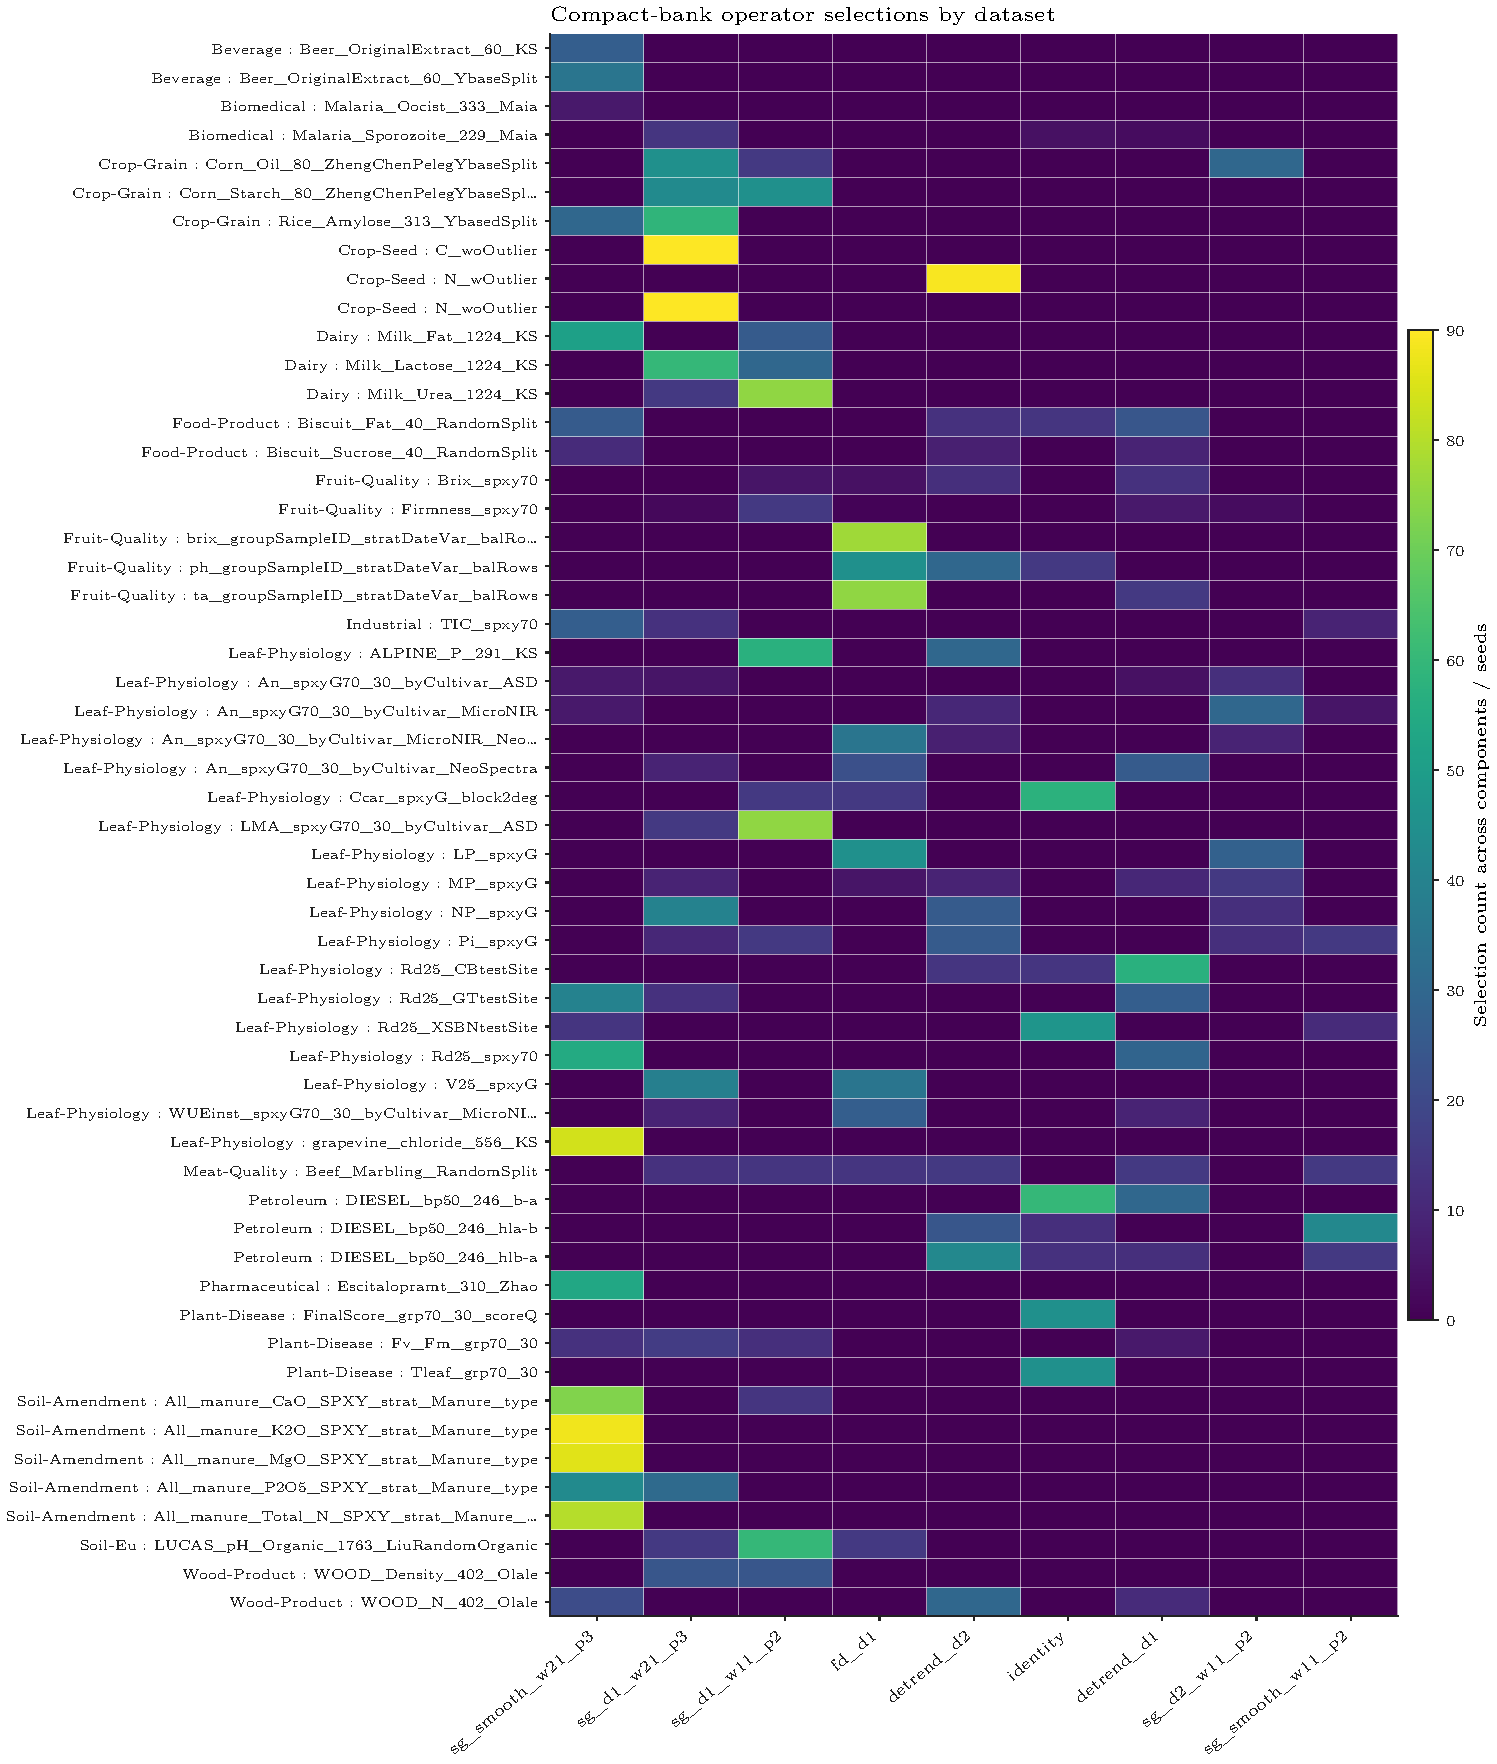
\includegraphics[width=\linewidth]{figures/fig_operator_heatmap.pdf}
  \caption{Per-dataset compact-bank operator heatmap.  Cells count selected
  components across compact AOM-PLS variants and seeds.}
  \label{fig:sup_operator_heatmap}
\end{figure}

\section{Full AOM-PLS Family}

The main manuscript reports the plain compact-CV5 AOM-PLS baseline.  It
promotes the ASLS compact-CV5 branch as the selected PLS regression variant.
Table \ref{tab:sup_aompls_family} keeps the full AOM-PLS and POP-PLS family in
the supplement.  Ratios are computed against PLS-standard on matching
dataset/seed rows.

\begin{table}[h]
\centering
\caption{AOM-PLS family summary from the seeds012 run.}
\label{tab:sup_aompls_family}
\small
\begin{tabularx}{\linewidth}{Xrrrrr}
\toprule
Variant & Datasets & Runs & Median RMSEP & Median ratio & Wins vs PLS \\
\midrule
ASLS-AOM-compact-cv5-numpy & 53 & 159 & 0.466 & 0.962 & 107/159 \\
AOM-compact-cv3-numpy & 55 & 165 & 0.442 & 0.980 & 98/165 \\
AOM-compact-cv5-numpy & 55 & 165 & 0.442 & 0.981 & 107/165 \\
AOM-compact-simpls-covariance-numpy & 55 & 165 & 0.795 & 0.999 & 84/165 \\
AOM-default-nipals-adjoint-numpy & 55 & 165 & 0.549 & 0.999 & 81/165 \\
nirs4all-AOM-PLS-default & 55 & 165 & 0.549 & 0.999 & 81/165 \\
PLS-standard-numpy & 55 & 165 & 0.795 & 1.000 & 0/165 \\
POP-nipals-adjoint-numpy & 55 & 165 & 1.784 & 1.373 & 34/165 \\
POP-simpls-covariance-numpy & 55 & 165 & 1.805 & 1.385 & 33/165 \\
\bottomrule
\end{tabularx}

\end{table}

The strict compact CV variants are close to the ASLS branch, but the ASLS
branch has the best aggregate RMSEP ratio among the reported AOM-PLS rows.
The default NIPALS-adjoint row is neutral at the aggregate level.  POP
regression variants are substantially weaker and are discussed separately
below.

\section{Full AOM-Ridge Family}

The Ridge family includes headline Blender and AutoSelect rows, plus local
and multi-branch variants.  Table~\ref{tab:sup_aomridge_family} reports the
variant-level summary.  Absolute RMSEP medians are descriptive only; the main
choice is based on paired ratios and wins.

\begin{table}[h]
\centering
\caption{AOM-Ridge family summary.}
\label{tab:sup_aomridge_family}
\small
\begin{tabularx}{\linewidth}{L{0.13\linewidth}Xrrrr}
\toprule
Source & Variant & Datasets & Runs & Median RMSEP & Median fit (s) \\
\midrule
headline & AOMRidge-global-compact-none & 53 & 53 & 0.359 & 21.60 \\
headline & AOMRidge-global-compact-none-asls & 53 & 53 & 0.382 & 24.35 \\
headline & AOMRidge-global-compact-none-snv & 53 & 53 & 0.389 & 18.23 \\
headline & AOM-PLS-compact-CV & 53 & 53 & 0.414 & 1.94 \\
headline & AOMRidgePLS-compact-colscale-cv-relative & 53 & 53 & 0.414 & 33.41 \\
headline & AOMRidge-Blender-headline-spxy3 & 53 & 55 & 0.471 & 960.1 \\
headline & AOMRidge-global-compact-none-msc & 53 & 53 & 0.483 & 25.90 \\
headline & AOMRidge-AutoSelect-headline-spxy3 & 53 & 55 & 0.520 & 646.2 \\
headline & Ridge-raw & 53 & 53 & 0.537 & 1.01 \\
headline & AOMRidgePLS-compact-Hmax-relative-emsc2 & 53 & 53 & 1.981 & 29.96 \\
seeds012 & AOMRidge-global-compact-none-split\_aware & 25 & 75 & 0.371 & 24.68 \\
seeds012 & AOMRidge-Local-compact-cv-blended & 25 & 75 & 0.484 & 4.19 \\
seeds012 & AOMRidge-Local-compact-knn50 & 25 & 75 & 0.523 & 3.19 \\
seeds012 & Ridge-raw & 25 & 76 & 0.571 & 0.49 \\
seeds012 & AOMRidge-MultiBranchMKL-compact-shrink03 & 25 & 75 & 3.599 & 101.2 \\
\bottomrule
\end{tabularx}

\end{table}

The global compact row is the plain Ridge AOM baseline used in the main text.
Blender is promoted as the selected Ridge variant because it gives the best
paired Ridge result against default Ridge and Ridge-HPO.  AutoSelect has a
similar median ratio against Ridge-HPO but fewer wins.  Local selectors are
fast and useful diagnostically, but they do not beat Ridge-HPO in the paired
summary.

\section{FastAOM Exploration}

FastAOM remains a supplementary exploration.  It tests whether low-rank
screening and sparse kernel mixtures can explore a larger operator-chain
space without fitting every chain as a full external pipeline.

\begin{table}[h]
\centering
\caption{FastAOM wide seed0 summary.  Each row reports its own available
complete datasets and is not the main $N_{\cap}=32$ paired denominator.}
\label{tab:sup_fastaom_variants}
\small
\begin{tabularx}{\linewidth}{p{0.38\linewidth}lrrrr}
\toprule
Variant & Family & $N$ & Median rel. RMSEP & Median fit (s) & Wins \\
\midrule
FastAOM-\allowbreak{}sparse-\allowbreak{}mkr-\allowbreak{}supervised & Sparse MKR & 50 & 1.009 & 87.77 & 10 \\
ASLS-\allowbreak{}AOM-\allowbreak{}compact-\allowbreak{}cv5-\allowbreak{}numpy & Reference & 57 & 1.011 & 1.36 & 8 \\
AOM-\allowbreak{}compact-\allowbreak{}cv5-\allowbreak{}numpy & Reference & 59 & 1.021 & 1.31 & 2 \\
FastAOM-\allowbreak{}sparse-\allowbreak{}mkr-\allowbreak{}compact & Sparse MKR & 50 & 1.022 & 2.48 & 3 \\
aom\_nirs-\allowbreak{}AOM-\allowbreak{}PLS-\allowbreak{}default & Reference & 59 & 1.034 & 0.97 & 7 \\
FastAOM-\allowbreak{}single-\allowbreak{}chain-\allowbreak{}compact & Single chain & 52 & 1.052 & 1.86 & 2 \\
FastAOM-\allowbreak{}single-\allowbreak{}chain-\allowbreak{}compact-\allowbreak{}cv5-\allowbreak{}numpy & Single chain & 52 & 1.052 & 2.02 & 0 \\
PLS-\allowbreak{}standard-\allowbreak{}numpy & Reference & 59 & 1.053 & 0.03 & 2 \\
FastAOM-\allowbreak{}soft-\allowbreak{}chain-\allowbreak{}compact & Soft chain & 52 & 1.062 & 3.05 & 1 \\
FastAOM-\allowbreak{}hard-\allowbreak{}chain-\allowbreak{}osc & Hard chain & 52 & 1.078 & 2.68 & 0 \\
FastAOM-\allowbreak{}hard-\allowbreak{}chain-\allowbreak{}supervised & Hard chain & 52 & 1.084 & 121.87 & 4 \\
FastAOM-\allowbreak{}hard-\allowbreak{}chain-\allowbreak{}asls & Hard chain & 52 & 1.105 & 174.46 & 3 \\
FastAOM-\allowbreak{}hard-\allowbreak{}chain-\allowbreak{}multibase & Hard chain & 52 & 1.109 & 5.62 & 0 \\
FastAOM-\allowbreak{}hard-\allowbreak{}chain-\allowbreak{}compact & Hard chain & 52 & 1.128 & 2.88 & 3 \\
FastAOM-\allowbreak{}single-\allowbreak{}chain-\allowbreak{}supervised-\allowbreak{}cv5-\allowbreak{}numpy & Single chain & 52 & 1.208 & 119.19 & 2 \\
FastAOM-\allowbreak{}hard-\allowbreak{}chain-\allowbreak{}compact-\allowbreak{}d4 & Hard chain & 1 & 1.256 & 38.08 & 0 \\
\bottomrule
\end{tabularx}

\end{table}

The best FastAOM entry by median relative RMSEP after the $N\ge50$ filter is
\code{FastAOM-sparse-mkr-supervised}: $N=50$, median relative RMSEP 1.009,
10 headline wins and median fit time 87.77 s.  The compact sparse-MKR variant
has median relative RMSEP 1.022 with median fit time 2.48 s.  The compact
single-chain variant has median relative RMSEP 1.052 and median fit time
1.86 s.  These rows show that screened operator-chain models are promising,
but the refreshed paired comparison does not beat the selected ASLS-AOM
variant on the same wide table.

\begin{figure}[h]
  \centering
  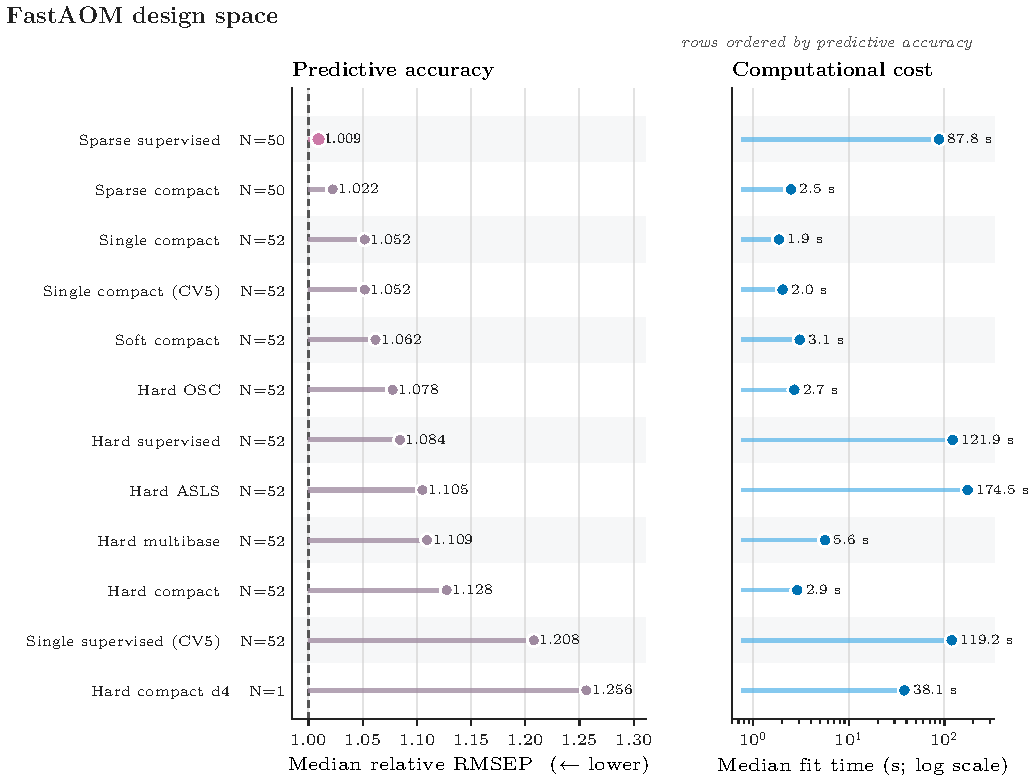
\includegraphics[width=\linewidth]{figures/fig_fastaom_variants.pdf}
  \caption{FastAOM variant comparison ordered by median relative RMSEP.  The
  upper axis shows median fit time on a logarithmic scale.}
\end{figure}

Hard-chain routing is valuable diagnostically because it assigns one chain
per latent component.  In the full table, however, the compact hard-chain
variant has median relative RMSEP 1.128, and the ASLS, multibase and
supervised hard-chain variants range from 1.084 to 1.109 with substantially
higher runtime for the supervised and ASLS branches.  These results explain
why FastAOM is not promoted in the main manuscript.

\section{POP-PLS Exploration}

POP-PLS allows different operators across components, which is attractive as
a modelling idea but weak in the current regression benchmark.  The two
regression POP variants have median ratios above 1.37 against PLS-standard
and win on roughly one fifth of dataset/seed rows.

\begin{table}[h]
\centering
\caption{POP-PLS regression summary from the AOM-PLS seeds012 run.}
\label{tab:sup_pop}
\small
\begin{tabularx}{\linewidth}{Xrrrr}
\toprule
POP variant & Datasets & Runs & Median ratio vs PLS & Wins vs PLS \\
\midrule
POP-nipals-adjoint-numpy & 55 & 165 & 1.373 & 34/165 \\
POP-simpls-covariance-numpy & 55 & 165 & 1.385 & 33/165 \\
\bottomrule
\end{tabularx}

\end{table}

The poor POP regression result is consistent with a noisy component-wise
selection surface: extra flexibility increases variance without producing a
stable aggregate gain.  POP-style classification rows are kept in the full
classification table, but POP is not part of the main result.

\section{Per-Dataset Regression Results}
\label{sec:sup_per_dataset_regression}

The heatmap gives a compact per-dataset view, and the long table gives the
underlying RMSEP values on the same $N_{\cap}=32$ regression rows used in the
main manuscript.

\begin{figure}[h]
  \centering
  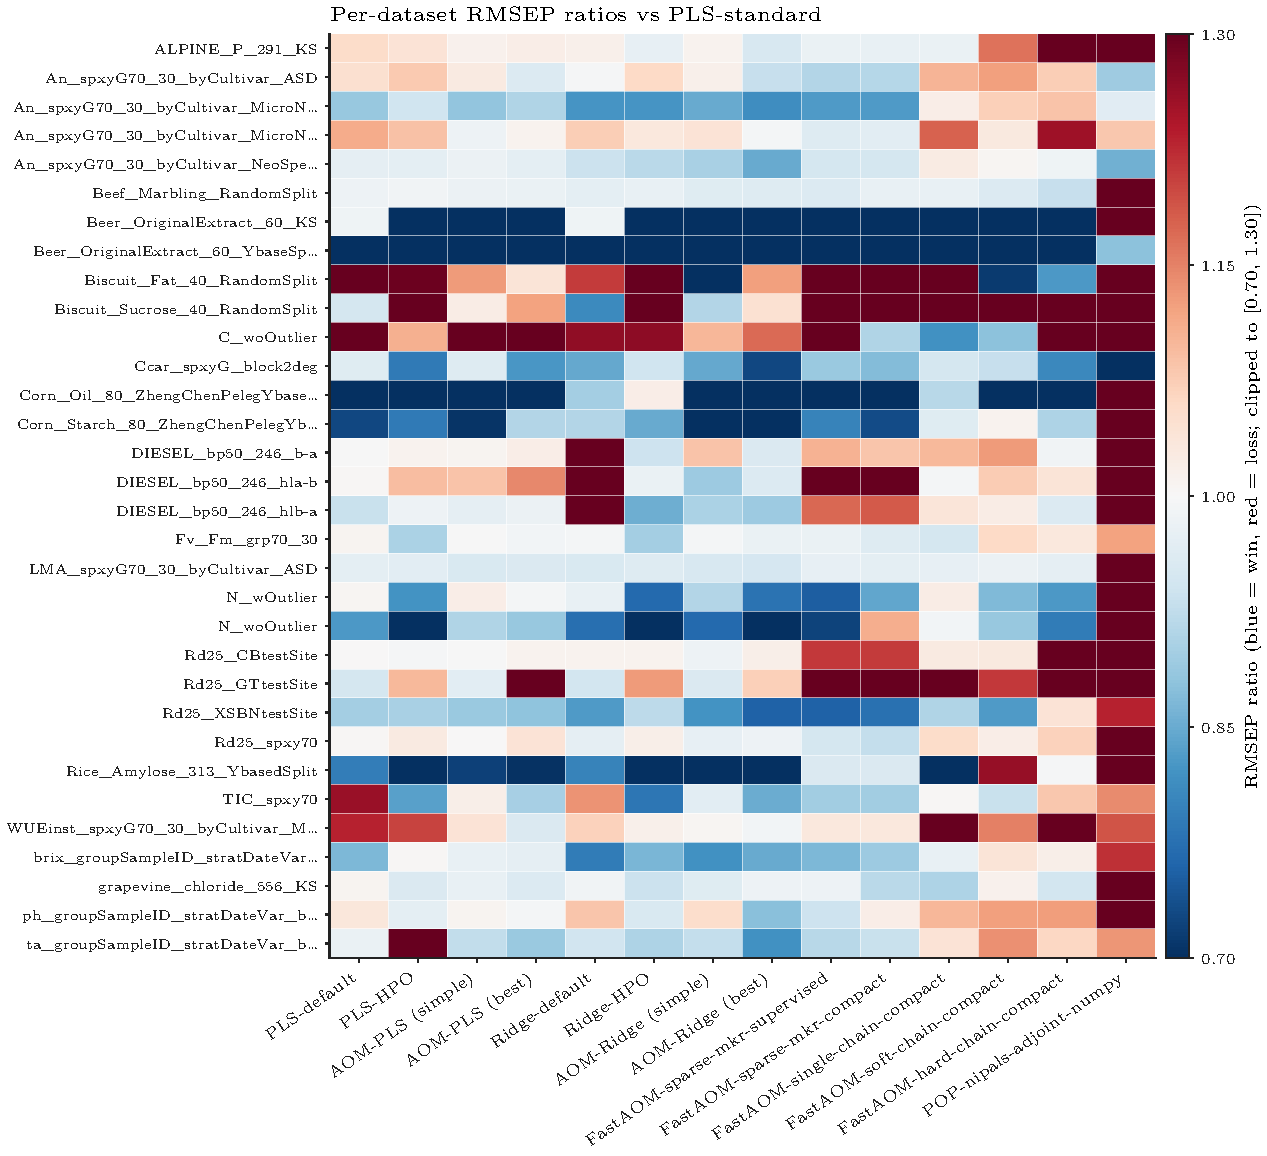
\includegraphics[width=\linewidth]{figures/fig_dataset_variant_heatmap.pdf}
  \caption{Per-dataset RMSEP ratios against PLS-standard.  Columns are ordered
  by PLS, AOM-PLS, Ridge, AOM-Ridge and then exploratory FastAOM/POP variants;
  missing cells are shown in light gray.}
  \label{fig:sup_dataset_heatmap}
\end{figure}

\clearpage
\begin{landscape}
\begingroup
\small
\setlength{\tabcolsep}{3.0pt}
\renewcommand{\arraystretch}{1.05}
\begin{longtable}{L{8.0cm}L{9.5cm}rr}
\caption{Per-dataset regression results on the strict intersection $N_{\cap}$ used in the paper.  Relative RMSEP is divided by PLS-standard on the same dataset when the denominator is finite.}\\
\toprule
Dataset & Variant & RMSEP & Rel. RMSEP \\
\midrule
\endfirsthead
\toprule
Dataset & Variant & RMSEP & Rel. RMSEP \\
\midrule
\endhead
ALPINE\_\allowbreak{}P\_\allowbreak{}291\_\allowbreak{}KS & PLS-\allowbreak{}standard-\allowbreak{}numpy & 0.05969 & 1.000 \\
ALPINE\_\allowbreak{}P\_\allowbreak{}291\_\allowbreak{}KS & AOM-\allowbreak{}compact-\allowbreak{}cv5-\allowbreak{}numpy & 0.06079 & 1.018 \\
ALPINE\_\allowbreak{}P\_\allowbreak{}291\_\allowbreak{}KS & ASLS-\allowbreak{}AOM-\allowbreak{}compact-\allowbreak{}cv5-\allowbreak{}numpy & 0.0606 & 1.015 \\
ALPINE\_\allowbreak{}P\_\allowbreak{}291\_\allowbreak{}KS & AOM-\allowbreak{}default-\allowbreak{}nipals-\allowbreak{}adjoint-\allowbreak{}numpy & 0.06733 & 1.128 \\
ALPINE\_\allowbreak{}P\_\allowbreak{}291\_\allowbreak{}KS & nirs4all-\allowbreak{}AOM-\allowbreak{}PLS-\allowbreak{}default & 0.06733 & 1.128 \\
ALPINE\_\allowbreak{}P\_\allowbreak{}291\_\allowbreak{}KS & FastAOM-\allowbreak{}sparse-\allowbreak{}mkr-\allowbreak{}supervised & 0.05844 & 0.979 \\
ALPINE\_\allowbreak{}P\_\allowbreak{}291\_\allowbreak{}KS & FastAOM-\allowbreak{}sparse-\allowbreak{}mkr-\allowbreak{}compact & 0.05843 & 0.979 \\
ALPINE\_\allowbreak{}P\_\allowbreak{}291\_\allowbreak{}KS & FastAOM-\allowbreak{}single-\allowbreak{}chain-\allowbreak{}compact & 0.05846 & 0.979 \\
ALPINE\_\allowbreak{}P\_\allowbreak{}291\_\allowbreak{}KS & FastAOM-\allowbreak{}soft-\allowbreak{}chain-\allowbreak{}compact & 0.06937 & 1.162 \\
ALPINE\_\allowbreak{}P\_\allowbreak{}291\_\allowbreak{}KS & FastAOM-\allowbreak{}hard-\allowbreak{}chain-\allowbreak{}compact & 0.07823 & 1.311 \\
ALPINE\_\allowbreak{}P\_\allowbreak{}291\_\allowbreak{}KS & FastAOM-\allowbreak{}hard-\allowbreak{}chain-\allowbreak{}osc & 0.07513 & 1.259 \\
ALPINE\_\allowbreak{}P\_\allowbreak{}291\_\allowbreak{}KS & FastAOM-\allowbreak{}hard-\allowbreak{}chain-\allowbreak{}asls & 0.07621 & 1.277 \\
ALPINE\_\allowbreak{}P\_\allowbreak{}291\_\allowbreak{}KS & FastAOM-\allowbreak{}hard-\allowbreak{}chain-\allowbreak{}multibase & 0.08579 & 1.437 \\
ALPINE\_\allowbreak{}P\_\allowbreak{}291\_\allowbreak{}KS & FastAOM-\allowbreak{}hard-\allowbreak{}chain-\allowbreak{}supervised & 0.07941 & 1.330 \\
ALPINE\_\allowbreak{}P\_\allowbreak{}291\_\allowbreak{}KS & POP-\allowbreak{}nipals-\allowbreak{}adjoint-\allowbreak{}numpy & 0.1007 & 1.687 \\
ALPINE\_\allowbreak{}P\_\allowbreak{}291\_\allowbreak{}KS & nirs4all-\allowbreak{}POP-\allowbreak{}PLS-\allowbreak{}default & 0.4153 & 6.957 \\
An\_\allowbreak{}spxyG70\_\allowbreak{}30\_\allowbreak{}byCultivar\_\allowbreak{}ASD & PLS-\allowbreak{}standard-\allowbreak{}numpy & 3.868 & 1.000 \\
An\_\allowbreak{}spxyG70\_\allowbreak{}30\_\allowbreak{}byCultivar\_\allowbreak{}ASD & AOM-\allowbreak{}compact-\allowbreak{}cv5-\allowbreak{}numpy & 4.078 & 1.054 \\
An\_\allowbreak{}spxyG70\_\allowbreak{}30\_\allowbreak{}byCultivar\_\allowbreak{}ASD & ASLS-\allowbreak{}AOM-\allowbreak{}compact-\allowbreak{}cv5-\allowbreak{}numpy & 3.791 & 0.980 \\
An\_\allowbreak{}spxyG70\_\allowbreak{}30\_\allowbreak{}byCultivar\_\allowbreak{}ASD & AOM-\allowbreak{}default-\allowbreak{}nipals-\allowbreak{}adjoint-\allowbreak{}numpy & 3.904 & 1.009 \\
An\_\allowbreak{}spxyG70\_\allowbreak{}30\_\allowbreak{}byCultivar\_\allowbreak{}ASD & nirs4all-\allowbreak{}AOM-\allowbreak{}PLS-\allowbreak{}default & 3.904 & 1.009 \\
An\_\allowbreak{}spxyG70\_\allowbreak{}30\_\allowbreak{}byCultivar\_\allowbreak{}ASD & FastAOM-\allowbreak{}sparse-\allowbreak{}mkr-\allowbreak{}supervised & 3.524 & 0.911 \\
An\_\allowbreak{}spxyG70\_\allowbreak{}30\_\allowbreak{}byCultivar\_\allowbreak{}ASD & FastAOM-\allowbreak{}sparse-\allowbreak{}mkr-\allowbreak{}compact & 3.539 & 0.915 \\
An\_\allowbreak{}spxyG70\_\allowbreak{}30\_\allowbreak{}byCultivar\_\allowbreak{}ASD & FastAOM-\allowbreak{}single-\allowbreak{}chain-\allowbreak{}compact & 4.264 & 1.102 \\
An\_\allowbreak{}spxyG70\_\allowbreak{}30\_\allowbreak{}byCultivar\_\allowbreak{}ASD & FastAOM-\allowbreak{}soft-\allowbreak{}chain-\allowbreak{}compact & 4.339 & 1.122 \\
An\_\allowbreak{}spxyG70\_\allowbreak{}30\_\allowbreak{}byCultivar\_\allowbreak{}ASD & FastAOM-\allowbreak{}hard-\allowbreak{}chain-\allowbreak{}compact & 4.15 & 1.073 \\
An\_\allowbreak{}spxyG70\_\allowbreak{}30\_\allowbreak{}byCultivar\_\allowbreak{}ASD & FastAOM-\allowbreak{}hard-\allowbreak{}chain-\allowbreak{}osc & 4.788 & 1.238 \\
An\_\allowbreak{}spxyG70\_\allowbreak{}30\_\allowbreak{}byCultivar\_\allowbreak{}ASD & FastAOM-\allowbreak{}hard-\allowbreak{}chain-\allowbreak{}asls & 3.943 & 1.019 \\
An\_\allowbreak{}spxyG70\_\allowbreak{}30\_\allowbreak{}byCultivar\_\allowbreak{}ASD & FastAOM-\allowbreak{}hard-\allowbreak{}chain-\allowbreak{}multibase & 5.477 & 1.416 \\
An\_\allowbreak{}spxyG70\_\allowbreak{}30\_\allowbreak{}byCultivar\_\allowbreak{}ASD & FastAOM-\allowbreak{}hard-\allowbreak{}chain-\allowbreak{}supervised & 4.323 & 1.118 \\
An\_\allowbreak{}spxyG70\_\allowbreak{}30\_\allowbreak{}byCultivar\_\allowbreak{}ASD & POP-\allowbreak{}nipals-\allowbreak{}adjoint-\allowbreak{}numpy & 3.451 & 0.892 \\
An\_\allowbreak{}spxyG70\_\allowbreak{}30\_\allowbreak{}byCultivar\_\allowbreak{}ASD & nirs4all-\allowbreak{}POP-\allowbreak{}PLS-\allowbreak{}default & 23.61 & 6.105 \\
An\_\allowbreak{}spxyG70\_\allowbreak{}30\_\allowbreak{}byCultivar\_\allowbreak{}MicroNIR & PLS-\allowbreak{}standard-\allowbreak{}numpy & 4.315 & 1.000 \\
An\_\allowbreak{}spxyG70\_\allowbreak{}30\_\allowbreak{}byCultivar\_\allowbreak{}MicroNIR & AOM-\allowbreak{}compact-\allowbreak{}cv5-\allowbreak{}numpy & 3.526 & 0.817 \\
An\_\allowbreak{}spxyG70\_\allowbreak{}30\_\allowbreak{}byCultivar\_\allowbreak{}MicroNIR & ASLS-\allowbreak{}AOM-\allowbreak{}compact-\allowbreak{}cv5-\allowbreak{}numpy & 3.622 & 0.840 \\
An\_\allowbreak{}spxyG70\_\allowbreak{}30\_\allowbreak{}byCultivar\_\allowbreak{}MicroNIR & AOM-\allowbreak{}default-\allowbreak{}nipals-\allowbreak{}adjoint-\allowbreak{}numpy & 4.343 & 1.006 \\
An\_\allowbreak{}spxyG70\_\allowbreak{}30\_\allowbreak{}byCultivar\_\allowbreak{}MicroNIR & nirs4all-\allowbreak{}AOM-\allowbreak{}PLS-\allowbreak{}default & 4.343 & 1.006 \\
An\_\allowbreak{}spxyG70\_\allowbreak{}30\_\allowbreak{}byCultivar\_\allowbreak{}MicroNIR & FastAOM-\allowbreak{}sparse-\allowbreak{}mkr-\allowbreak{}supervised & 3.586 & 0.831 \\
An\_\allowbreak{}spxyG70\_\allowbreak{}30\_\allowbreak{}byCultivar\_\allowbreak{}MicroNIR & FastAOM-\allowbreak{}sparse-\allowbreak{}mkr-\allowbreak{}compact & 3.586 & 0.831 \\
An\_\allowbreak{}spxyG70\_\allowbreak{}30\_\allowbreak{}byCultivar\_\allowbreak{}MicroNIR & FastAOM-\allowbreak{}single-\allowbreak{}chain-\allowbreak{}compact & 4.404 & 1.021 \\
An\_\allowbreak{}spxyG70\_\allowbreak{}30\_\allowbreak{}byCultivar\_\allowbreak{}MicroNIR & FastAOM-\allowbreak{}soft-\allowbreak{}chain-\allowbreak{}compact & 4.627 & 1.072 \\
An\_\allowbreak{}spxyG70\_\allowbreak{}30\_\allowbreak{}byCultivar\_\allowbreak{}MicroNIR & FastAOM-\allowbreak{}hard-\allowbreak{}chain-\allowbreak{}compact & 4.685 & 1.086 \\
An\_\allowbreak{}spxyG70\_\allowbreak{}30\_\allowbreak{}byCultivar\_\allowbreak{}MicroNIR & FastAOM-\allowbreak{}hard-\allowbreak{}chain-\allowbreak{}osc & 4.809 & 1.115 \\
An\_\allowbreak{}spxyG70\_\allowbreak{}30\_\allowbreak{}byCultivar\_\allowbreak{}MicroNIR & FastAOM-\allowbreak{}hard-\allowbreak{}chain-\allowbreak{}asls & 5.084 & 1.178 \\
An\_\allowbreak{}spxyG70\_\allowbreak{}30\_\allowbreak{}byCultivar\_\allowbreak{}MicroNIR & FastAOM-\allowbreak{}hard-\allowbreak{}chain-\allowbreak{}multibase & 4.947 & 1.146 \\
An\_\allowbreak{}spxyG70\_\allowbreak{}30\_\allowbreak{}byCultivar\_\allowbreak{}MicroNIR & FastAOM-\allowbreak{}hard-\allowbreak{}chain-\allowbreak{}supervised & 4.678 & 1.084 \\
An\_\allowbreak{}spxyG70\_\allowbreak{}30\_\allowbreak{}byCultivar\_\allowbreak{}MicroNIR & POP-\allowbreak{}nipals-\allowbreak{}adjoint-\allowbreak{}numpy & 4.166 & 0.966 \\
An\_\allowbreak{}spxyG70\_\allowbreak{}30\_\allowbreak{}byCultivar\_\allowbreak{}MicroNIR & nirs4all-\allowbreak{}POP-\allowbreak{}PLS-\allowbreak{}default & 21.22 & 4.919 \\
An\_\allowbreak{}spxyG70\_\allowbreak{}30\_\allowbreak{}byCultivar\_\allowbreak{}MicroNIR\_\allowbreak{}NeoSpectra & PLS-\allowbreak{}standard-\allowbreak{}numpy & 3.863 & 1.000 \\
An\_\allowbreak{}spxyG70\_\allowbreak{}30\_\allowbreak{}byCultivar\_\allowbreak{}MicroNIR\_\allowbreak{}NeoSpectra & AOM-\allowbreak{}compact-\allowbreak{}cv5-\allowbreak{}numpy & 3.791 & 0.981 \\
An\_\allowbreak{}spxyG70\_\allowbreak{}30\_\allowbreak{}byCultivar\_\allowbreak{}MicroNIR\_\allowbreak{}NeoSpectra & ASLS-\allowbreak{}AOM-\allowbreak{}compact-\allowbreak{}cv5-\allowbreak{}numpy & 3.618 & 0.936 \\
An\_\allowbreak{}spxyG70\_\allowbreak{}30\_\allowbreak{}byCultivar\_\allowbreak{}MicroNIR\_\allowbreak{}NeoSpectra & AOM-\allowbreak{}default-\allowbreak{}nipals-\allowbreak{}adjoint-\allowbreak{}numpy & 4.353 & 1.127 \\
An\_\allowbreak{}spxyG70\_\allowbreak{}30\_\allowbreak{}byCultivar\_\allowbreak{}MicroNIR\_\allowbreak{}NeoSpectra & nirs4all-\allowbreak{}AOM-\allowbreak{}PLS-\allowbreak{}default & 4.353 & 1.127 \\
An\_\allowbreak{}spxyG70\_\allowbreak{}30\_\allowbreak{}byCultivar\_\allowbreak{}MicroNIR\_\allowbreak{}NeoSpectra & FastAOM-\allowbreak{}sparse-\allowbreak{}mkr-\allowbreak{}supervised & 3.712 & 0.961 \\
An\_\allowbreak{}spxyG70\_\allowbreak{}30\_\allowbreak{}byCultivar\_\allowbreak{}MicroNIR\_\allowbreak{}NeoSpectra & FastAOM-\allowbreak{}sparse-\allowbreak{}mkr-\allowbreak{}compact & 3.74 & 0.968 \\
An\_\allowbreak{}spxyG70\_\allowbreak{}30\_\allowbreak{}byCultivar\_\allowbreak{}MicroNIR\_\allowbreak{}NeoSpectra & FastAOM-\allowbreak{}single-\allowbreak{}chain-\allowbreak{}compact & 4.549 & 1.178 \\
An\_\allowbreak{}spxyG70\_\allowbreak{}30\_\allowbreak{}byCultivar\_\allowbreak{}MicroNIR\_\allowbreak{}NeoSpectra & FastAOM-\allowbreak{}soft-\allowbreak{}chain-\allowbreak{}compact & 3.972 & 1.028 \\
An\_\allowbreak{}spxyG70\_\allowbreak{}30\_\allowbreak{}byCultivar\_\allowbreak{}MicroNIR\_\allowbreak{}NeoSpectra & FastAOM-\allowbreak{}hard-\allowbreak{}chain-\allowbreak{}compact & 4.842 & 1.253 \\
An\_\allowbreak{}spxyG70\_\allowbreak{}30\_\allowbreak{}byCultivar\_\allowbreak{}MicroNIR\_\allowbreak{}NeoSpectra & FastAOM-\allowbreak{}hard-\allowbreak{}chain-\allowbreak{}osc & 4.295 & 1.112 \\
An\_\allowbreak{}spxyG70\_\allowbreak{}30\_\allowbreak{}byCultivar\_\allowbreak{}MicroNIR\_\allowbreak{}NeoSpectra & FastAOM-\allowbreak{}hard-\allowbreak{}chain-\allowbreak{}asls & 4.858 & 1.257 \\
An\_\allowbreak{}spxyG70\_\allowbreak{}30\_\allowbreak{}byCultivar\_\allowbreak{}MicroNIR\_\allowbreak{}NeoSpectra & FastAOM-\allowbreak{}hard-\allowbreak{}chain-\allowbreak{}multibase & 5.064 & 1.311 \\
An\_\allowbreak{}spxyG70\_\allowbreak{}30\_\allowbreak{}byCultivar\_\allowbreak{}MicroNIR\_\allowbreak{}NeoSpectra & FastAOM-\allowbreak{}hard-\allowbreak{}chain-\allowbreak{}supervised & 4.586 & 1.187 \\
An\_\allowbreak{}spxyG70\_\allowbreak{}30\_\allowbreak{}byCultivar\_\allowbreak{}MicroNIR\_\allowbreak{}NeoSpectra & POP-\allowbreak{}nipals-\allowbreak{}adjoint-\allowbreak{}numpy & 4.177 & 1.081 \\
An\_\allowbreak{}spxyG70\_\allowbreak{}30\_\allowbreak{}byCultivar\_\allowbreak{}MicroNIR\_\allowbreak{}NeoSpectra & nirs4all-\allowbreak{}POP-\allowbreak{}PLS-\allowbreak{}default & 22.44 & 5.808 \\
An\_\allowbreak{}spxyG70\_\allowbreak{}30\_\allowbreak{}byCultivar\_\allowbreak{}NeoSpectra & PLS-\allowbreak{}standard-\allowbreak{}numpy & 5.198 & 1.000 \\
An\_\allowbreak{}spxyG70\_\allowbreak{}30\_\allowbreak{}byCultivar\_\allowbreak{}NeoSpectra & AOM-\allowbreak{}compact-\allowbreak{}cv5-\allowbreak{}numpy & 5.156 & 0.992 \\
An\_\allowbreak{}spxyG70\_\allowbreak{}30\_\allowbreak{}byCultivar\_\allowbreak{}NeoSpectra & ASLS-\allowbreak{}AOM-\allowbreak{}compact-\allowbreak{}cv5-\allowbreak{}numpy & 4.978 & 0.958 \\
An\_\allowbreak{}spxyG70\_\allowbreak{}30\_\allowbreak{}byCultivar\_\allowbreak{}NeoSpectra & AOM-\allowbreak{}default-\allowbreak{}nipals-\allowbreak{}adjoint-\allowbreak{}numpy & 5.525 & 1.063 \\
An\_\allowbreak{}spxyG70\_\allowbreak{}30\_\allowbreak{}byCultivar\_\allowbreak{}NeoSpectra & nirs4all-\allowbreak{}AOM-\allowbreak{}PLS-\allowbreak{}default & 5.525 & 1.063 \\
An\_\allowbreak{}spxyG70\_\allowbreak{}30\_\allowbreak{}byCultivar\_\allowbreak{}NeoSpectra & FastAOM-\allowbreak{}sparse-\allowbreak{}mkr-\allowbreak{}supervised & 4.929 & 0.948 \\
An\_\allowbreak{}spxyG70\_\allowbreak{}30\_\allowbreak{}byCultivar\_\allowbreak{}NeoSpectra & FastAOM-\allowbreak{}sparse-\allowbreak{}mkr-\allowbreak{}compact & 4.929 & 0.948 \\
An\_\allowbreak{}spxyG70\_\allowbreak{}30\_\allowbreak{}byCultivar\_\allowbreak{}NeoSpectra & FastAOM-\allowbreak{}single-\allowbreak{}chain-\allowbreak{}compact & 5.322 & 1.024 \\
An\_\allowbreak{}spxyG70\_\allowbreak{}30\_\allowbreak{}byCultivar\_\allowbreak{}NeoSpectra & FastAOM-\allowbreak{}soft-\allowbreak{}chain-\allowbreak{}compact & 5.232 & 1.007 \\
An\_\allowbreak{}spxyG70\_\allowbreak{}30\_\allowbreak{}byCultivar\_\allowbreak{}NeoSpectra & FastAOM-\allowbreak{}hard-\allowbreak{}chain-\allowbreak{}compact & 5.125 & 0.986 \\
An\_\allowbreak{}spxyG70\_\allowbreak{}30\_\allowbreak{}byCultivar\_\allowbreak{}NeoSpectra & FastAOM-\allowbreak{}hard-\allowbreak{}chain-\allowbreak{}osc & 5.125 & 0.986 \\
An\_\allowbreak{}spxyG70\_\allowbreak{}30\_\allowbreak{}byCultivar\_\allowbreak{}NeoSpectra & FastAOM-\allowbreak{}hard-\allowbreak{}chain-\allowbreak{}asls & 5.223 & 1.005 \\
An\_\allowbreak{}spxyG70\_\allowbreak{}30\_\allowbreak{}byCultivar\_\allowbreak{}NeoSpectra & FastAOM-\allowbreak{}hard-\allowbreak{}chain-\allowbreak{}multibase & 5.277 & 1.015 \\
An\_\allowbreak{}spxyG70\_\allowbreak{}30\_\allowbreak{}byCultivar\_\allowbreak{}NeoSpectra & FastAOM-\allowbreak{}hard-\allowbreak{}chain-\allowbreak{}supervised & 5.174 & 0.996 \\
An\_\allowbreak{}spxyG70\_\allowbreak{}30\_\allowbreak{}byCultivar\_\allowbreak{}NeoSpectra & POP-\allowbreak{}nipals-\allowbreak{}adjoint-\allowbreak{}numpy & 4.452 & 0.857 \\
An\_\allowbreak{}spxyG70\_\allowbreak{}30\_\allowbreak{}byCultivar\_\allowbreak{}NeoSpectra & nirs4all-\allowbreak{}POP-\allowbreak{}PLS-\allowbreak{}default & 66.16 & 12.730 \\
Beef\_\allowbreak{}Marbling\_\allowbreak{}RandomSplit & PLS-\allowbreak{}standard-\allowbreak{}numpy & 74.82 & 1.000 \\
Beef\_\allowbreak{}Marbling\_\allowbreak{}RandomSplit & AOM-\allowbreak{}compact-\allowbreak{}cv5-\allowbreak{}numpy & 75.06 & 1.003 \\
Beef\_\allowbreak{}Marbling\_\allowbreak{}RandomSplit & ASLS-\allowbreak{}AOM-\allowbreak{}compact-\allowbreak{}cv5-\allowbreak{}numpy & 72.98 & 0.975 \\
Beef\_\allowbreak{}Marbling\_\allowbreak{}RandomSplit & AOM-\allowbreak{}default-\allowbreak{}nipals-\allowbreak{}adjoint-\allowbreak{}numpy & 72.78 & 0.973 \\
Beef\_\allowbreak{}Marbling\_\allowbreak{}RandomSplit & nirs4all-\allowbreak{}AOM-\allowbreak{}PLS-\allowbreak{}default & 72.78 & 0.973 \\
Beef\_\allowbreak{}Marbling\_\allowbreak{}RandomSplit & FastAOM-\allowbreak{}sparse-\allowbreak{}mkr-\allowbreak{}supervised & 71.74 & 0.959 \\
Beef\_\allowbreak{}Marbling\_\allowbreak{}RandomSplit & FastAOM-\allowbreak{}sparse-\allowbreak{}mkr-\allowbreak{}compact & 73.08 & 0.977 \\
Beef\_\allowbreak{}Marbling\_\allowbreak{}RandomSplit & FastAOM-\allowbreak{}single-\allowbreak{}chain-\allowbreak{}compact & 73.12 & 0.977 \\
Beef\_\allowbreak{}Marbling\_\allowbreak{}RandomSplit & FastAOM-\allowbreak{}soft-\allowbreak{}chain-\allowbreak{}compact & 71.72 & 0.959 \\
Beef\_\allowbreak{}Marbling\_\allowbreak{}RandomSplit & FastAOM-\allowbreak{}hard-\allowbreak{}chain-\allowbreak{}compact & 69.62 & 0.930 \\
Beef\_\allowbreak{}Marbling\_\allowbreak{}RandomSplit & FastAOM-\allowbreak{}hard-\allowbreak{}chain-\allowbreak{}osc & 69.62 & 0.930 \\
Beef\_\allowbreak{}Marbling\_\allowbreak{}RandomSplit & FastAOM-\allowbreak{}hard-\allowbreak{}chain-\allowbreak{}asls & 71.2 & 0.952 \\
Beef\_\allowbreak{}Marbling\_\allowbreak{}RandomSplit & FastAOM-\allowbreak{}hard-\allowbreak{}chain-\allowbreak{}multibase & 71.82 & 0.960 \\
Beef\_\allowbreak{}Marbling\_\allowbreak{}RandomSplit & FastAOM-\allowbreak{}hard-\allowbreak{}chain-\allowbreak{}supervised & 72.7 & 0.972 \\
Beef\_\allowbreak{}Marbling\_\allowbreak{}RandomSplit & POP-\allowbreak{}nipals-\allowbreak{}adjoint-\allowbreak{}numpy & 98.66 & 1.319 \\
Beef\_\allowbreak{}Marbling\_\allowbreak{}RandomSplit & nirs4all-\allowbreak{}POP-\allowbreak{}PLS-\allowbreak{}default & 564.5 & 7.544 \\
Beer\_\allowbreak{}OriginalExtract\_\allowbreak{}60\_\allowbreak{}KS & PLS-\allowbreak{}standard-\allowbreak{}numpy & 0.5784 & 1.000 \\
Beer\_\allowbreak{}OriginalExtract\_\allowbreak{}60\_\allowbreak{}KS & AOM-\allowbreak{}compact-\allowbreak{}cv5-\allowbreak{}numpy & 0.3289 & 0.569 \\
Beer\_\allowbreak{}OriginalExtract\_\allowbreak{}60\_\allowbreak{}KS & ASLS-\allowbreak{}AOM-\allowbreak{}compact-\allowbreak{}cv5-\allowbreak{}numpy & 0.2369 & 0.410 \\
Beer\_\allowbreak{}OriginalExtract\_\allowbreak{}60\_\allowbreak{}KS & AOM-\allowbreak{}default-\allowbreak{}nipals-\allowbreak{}adjoint-\allowbreak{}numpy & 0.2042 & 0.353 \\
Beer\_\allowbreak{}OriginalExtract\_\allowbreak{}60\_\allowbreak{}KS & nirs4all-\allowbreak{}AOM-\allowbreak{}PLS-\allowbreak{}default & 0.2042 & 0.353 \\
Beer\_\allowbreak{}OriginalExtract\_\allowbreak{}60\_\allowbreak{}KS & FastAOM-\allowbreak{}sparse-\allowbreak{}mkr-\allowbreak{}supervised & 0.1611 & 0.279 \\
Beer\_\allowbreak{}OriginalExtract\_\allowbreak{}60\_\allowbreak{}KS & FastAOM-\allowbreak{}sparse-\allowbreak{}mkr-\allowbreak{}compact & 0.1653 & 0.286 \\
Beer\_\allowbreak{}OriginalExtract\_\allowbreak{}60\_\allowbreak{}KS & FastAOM-\allowbreak{}single-\allowbreak{}chain-\allowbreak{}compact & 0.2382 & 0.412 \\
Beer\_\allowbreak{}OriginalExtract\_\allowbreak{}60\_\allowbreak{}KS & FastAOM-\allowbreak{}soft-\allowbreak{}chain-\allowbreak{}compact & 0.2384 & 0.412 \\
Beer\_\allowbreak{}OriginalExtract\_\allowbreak{}60\_\allowbreak{}KS & FastAOM-\allowbreak{}hard-\allowbreak{}chain-\allowbreak{}compact & 0.245 & 0.424 \\
Beer\_\allowbreak{}OriginalExtract\_\allowbreak{}60\_\allowbreak{}KS & FastAOM-\allowbreak{}hard-\allowbreak{}chain-\allowbreak{}osc & 0.2452 & 0.424 \\
Beer\_\allowbreak{}OriginalExtract\_\allowbreak{}60\_\allowbreak{}KS & FastAOM-\allowbreak{}hard-\allowbreak{}chain-\allowbreak{}asls & 0.2431 & 0.420 \\
Beer\_\allowbreak{}OriginalExtract\_\allowbreak{}60\_\allowbreak{}KS & FastAOM-\allowbreak{}hard-\allowbreak{}chain-\allowbreak{}multibase & 0.245 & 0.424 \\
Beer\_\allowbreak{}OriginalExtract\_\allowbreak{}60\_\allowbreak{}KS & FastAOM-\allowbreak{}hard-\allowbreak{}chain-\allowbreak{}supervised & 0.2449 & 0.423 \\
Beer\_\allowbreak{}OriginalExtract\_\allowbreak{}60\_\allowbreak{}KS & POP-\allowbreak{}nipals-\allowbreak{}adjoint-\allowbreak{}numpy & 1.624 & 2.809 \\
Beer\_\allowbreak{}OriginalExtract\_\allowbreak{}60\_\allowbreak{}KS & nirs4all-\allowbreak{}POP-\allowbreak{}PLS-\allowbreak{}default & 0.9814 & 1.697 \\
Beer\_\allowbreak{}OriginalExtract\_\allowbreak{}60\_\allowbreak{}YbaseSplit & PLS-\allowbreak{}standard-\allowbreak{}numpy & 0.9263 & 1.000 \\
Beer\_\allowbreak{}OriginalExtract\_\allowbreak{}60\_\allowbreak{}YbaseSplit & AOM-\allowbreak{}compact-\allowbreak{}cv5-\allowbreak{}numpy & 0.2793 & 0.302 \\
Beer\_\allowbreak{}OriginalExtract\_\allowbreak{}60\_\allowbreak{}YbaseSplit & ASLS-\allowbreak{}AOM-\allowbreak{}compact-\allowbreak{}cv5-\allowbreak{}numpy & 0.2538 & 0.274 \\
Beer\_\allowbreak{}OriginalExtract\_\allowbreak{}60\_\allowbreak{}YbaseSplit & AOM-\allowbreak{}default-\allowbreak{}nipals-\allowbreak{}adjoint-\allowbreak{}numpy & 0.2107 & 0.227 \\
Beer\_\allowbreak{}OriginalExtract\_\allowbreak{}60\_\allowbreak{}YbaseSplit & nirs4all-\allowbreak{}AOM-\allowbreak{}PLS-\allowbreak{}default & 0.2107 & 0.227 \\
Beer\_\allowbreak{}OriginalExtract\_\allowbreak{}60\_\allowbreak{}YbaseSplit & FastAOM-\allowbreak{}sparse-\allowbreak{}mkr-\allowbreak{}supervised & 0.2766 & 0.299 \\
Beer\_\allowbreak{}OriginalExtract\_\allowbreak{}60\_\allowbreak{}YbaseSplit & FastAOM-\allowbreak{}sparse-\allowbreak{}mkr-\allowbreak{}compact & 0.2713 & 0.293 \\
Beer\_\allowbreak{}OriginalExtract\_\allowbreak{}60\_\allowbreak{}YbaseSplit & FastAOM-\allowbreak{}single-\allowbreak{}chain-\allowbreak{}compact & 0.3005 & 0.324 \\
Beer\_\allowbreak{}OriginalExtract\_\allowbreak{}60\_\allowbreak{}YbaseSplit & FastAOM-\allowbreak{}soft-\allowbreak{}chain-\allowbreak{}compact & 0.3082 & 0.333 \\
Beer\_\allowbreak{}OriginalExtract\_\allowbreak{}60\_\allowbreak{}YbaseSplit & FastAOM-\allowbreak{}hard-\allowbreak{}chain-\allowbreak{}compact & 0.316 & 0.341 \\
Beer\_\allowbreak{}OriginalExtract\_\allowbreak{}60\_\allowbreak{}YbaseSplit & FastAOM-\allowbreak{}hard-\allowbreak{}chain-\allowbreak{}osc & 0.3182 & 0.344 \\
Beer\_\allowbreak{}OriginalExtract\_\allowbreak{}60\_\allowbreak{}YbaseSplit & FastAOM-\allowbreak{}hard-\allowbreak{}chain-\allowbreak{}asls & 0.3107 & 0.335 \\
Beer\_\allowbreak{}OriginalExtract\_\allowbreak{}60\_\allowbreak{}YbaseSplit & FastAOM-\allowbreak{}hard-\allowbreak{}chain-\allowbreak{}multibase & 0.3094 & 0.334 \\
Beer\_\allowbreak{}OriginalExtract\_\allowbreak{}60\_\allowbreak{}YbaseSplit & FastAOM-\allowbreak{}hard-\allowbreak{}chain-\allowbreak{}supervised & 0.3189 & 0.344 \\
Beer\_\allowbreak{}OriginalExtract\_\allowbreak{}60\_\allowbreak{}YbaseSplit & POP-\allowbreak{}nipals-\allowbreak{}adjoint-\allowbreak{}numpy & 0.8123 & 0.877 \\
Beer\_\allowbreak{}OriginalExtract\_\allowbreak{}60\_\allowbreak{}YbaseSplit & nirs4all-\allowbreak{}POP-\allowbreak{}PLS-\allowbreak{}default & 0.9859 & 1.064 \\
Biscuit\_\allowbreak{}Fat\_\allowbreak{}40\_\allowbreak{}RandomSplit & PLS-\allowbreak{}standard-\allowbreak{}numpy & 0.4197 & 1.000 \\
Biscuit\_\allowbreak{}Fat\_\allowbreak{}40\_\allowbreak{}RandomSplit & AOM-\allowbreak{}compact-\allowbreak{}cv5-\allowbreak{}numpy & 0.4421 & 1.054 \\
Biscuit\_\allowbreak{}Fat\_\allowbreak{}40\_\allowbreak{}RandomSplit & ASLS-\allowbreak{}AOM-\allowbreak{}compact-\allowbreak{}cv5-\allowbreak{}numpy & 0.4371 & 1.042 \\
Biscuit\_\allowbreak{}Fat\_\allowbreak{}40\_\allowbreak{}RandomSplit & AOM-\allowbreak{}default-\allowbreak{}nipals-\allowbreak{}adjoint-\allowbreak{}numpy & 0.5491 & 1.308 \\
Biscuit\_\allowbreak{}Fat\_\allowbreak{}40\_\allowbreak{}RandomSplit & nirs4all-\allowbreak{}AOM-\allowbreak{}PLS-\allowbreak{}default & 0.5491 & 1.308 \\
Biscuit\_\allowbreak{}Fat\_\allowbreak{}40\_\allowbreak{}RandomSplit & FastAOM-\allowbreak{}sparse-\allowbreak{}mkr-\allowbreak{}supervised & 0.5547 & 1.322 \\
Biscuit\_\allowbreak{}Fat\_\allowbreak{}40\_\allowbreak{}RandomSplit & FastAOM-\allowbreak{}sparse-\allowbreak{}mkr-\allowbreak{}compact & 0.5547 & 1.322 \\
Biscuit\_\allowbreak{}Fat\_\allowbreak{}40\_\allowbreak{}RandomSplit & FastAOM-\allowbreak{}single-\allowbreak{}chain-\allowbreak{}compact & 0.8011 & 1.909 \\
Biscuit\_\allowbreak{}Fat\_\allowbreak{}40\_\allowbreak{}RandomSplit & FastAOM-\allowbreak{}soft-\allowbreak{}chain-\allowbreak{}compact & 0.2989 & 0.712 \\
Biscuit\_\allowbreak{}Fat\_\allowbreak{}40\_\allowbreak{}RandomSplit & FastAOM-\allowbreak{}hard-\allowbreak{}chain-\allowbreak{}compact & 0.3477 & 0.828 \\
Biscuit\_\allowbreak{}Fat\_\allowbreak{}40\_\allowbreak{}RandomSplit & FastAOM-\allowbreak{}hard-\allowbreak{}chain-\allowbreak{}osc & 0.5561 & 1.325 \\
Biscuit\_\allowbreak{}Fat\_\allowbreak{}40\_\allowbreak{}RandomSplit & FastAOM-\allowbreak{}hard-\allowbreak{}chain-\allowbreak{}asls & 0.4015 & 0.957 \\
Biscuit\_\allowbreak{}Fat\_\allowbreak{}40\_\allowbreak{}RandomSplit & FastAOM-\allowbreak{}hard-\allowbreak{}chain-\allowbreak{}multibase & 0.5485 & 1.307 \\
Biscuit\_\allowbreak{}Fat\_\allowbreak{}40\_\allowbreak{}RandomSplit & FastAOM-\allowbreak{}hard-\allowbreak{}chain-\allowbreak{}supervised & 1.559 & 3.716 \\
Biscuit\_\allowbreak{}Fat\_\allowbreak{}40\_\allowbreak{}RandomSplit & POP-\allowbreak{}nipals-\allowbreak{}adjoint-\allowbreak{}numpy & 2.035 & 4.850 \\
Biscuit\_\allowbreak{}Fat\_\allowbreak{}40\_\allowbreak{}RandomSplit & nirs4all-\allowbreak{}POP-\allowbreak{}PLS-\allowbreak{}default & 5.867 & 13.979 \\
Biscuit\_\allowbreak{}Sucrose\_\allowbreak{}40\_\allowbreak{}RandomSplit & PLS-\allowbreak{}standard-\allowbreak{}numpy & 1.154 & 1.000 \\
Biscuit\_\allowbreak{}Sucrose\_\allowbreak{}40\_\allowbreak{}RandomSplit & AOM-\allowbreak{}compact-\allowbreak{}cv5-\allowbreak{}numpy & 1.165 & 1.009 \\
Biscuit\_\allowbreak{}Sucrose\_\allowbreak{}40\_\allowbreak{}RandomSplit & ASLS-\allowbreak{}AOM-\allowbreak{}compact-\allowbreak{}cv5-\allowbreak{}numpy & 0.8817 & 0.764 \\
Biscuit\_\allowbreak{}Sucrose\_\allowbreak{}40\_\allowbreak{}RandomSplit & AOM-\allowbreak{}default-\allowbreak{}nipals-\allowbreak{}adjoint-\allowbreak{}numpy & 4.347 & 3.765 \\
Biscuit\_\allowbreak{}Sucrose\_\allowbreak{}40\_\allowbreak{}RandomSplit & nirs4all-\allowbreak{}AOM-\allowbreak{}PLS-\allowbreak{}default & 4.347 & 3.765 \\
Biscuit\_\allowbreak{}Sucrose\_\allowbreak{}40\_\allowbreak{}RandomSplit & FastAOM-\allowbreak{}sparse-\allowbreak{}mkr-\allowbreak{}supervised & 4.516 & 3.912 \\
Biscuit\_\allowbreak{}Sucrose\_\allowbreak{}40\_\allowbreak{}RandomSplit & FastAOM-\allowbreak{}sparse-\allowbreak{}mkr-\allowbreak{}compact & 4.035 & 3.495 \\
Biscuit\_\allowbreak{}Sucrose\_\allowbreak{}40\_\allowbreak{}RandomSplit & FastAOM-\allowbreak{}single-\allowbreak{}chain-\allowbreak{}compact & 3.124 & 2.706 \\
Biscuit\_\allowbreak{}Sucrose\_\allowbreak{}40\_\allowbreak{}RandomSplit & FastAOM-\allowbreak{}soft-\allowbreak{}chain-\allowbreak{}compact & 3.35 & 2.901 \\
Biscuit\_\allowbreak{}Sucrose\_\allowbreak{}40\_\allowbreak{}RandomSplit & FastAOM-\allowbreak{}hard-\allowbreak{}chain-\allowbreak{}compact & 3.082 & 2.670 \\
Biscuit\_\allowbreak{}Sucrose\_\allowbreak{}40\_\allowbreak{}RandomSplit & FastAOM-\allowbreak{}hard-\allowbreak{}chain-\allowbreak{}osc & 2.486 & 2.153 \\
Biscuit\_\allowbreak{}Sucrose\_\allowbreak{}40\_\allowbreak{}RandomSplit & FastAOM-\allowbreak{}hard-\allowbreak{}chain-\allowbreak{}asls & 3.29 & 2.850 \\
Biscuit\_\allowbreak{}Sucrose\_\allowbreak{}40\_\allowbreak{}RandomSplit & FastAOM-\allowbreak{}hard-\allowbreak{}chain-\allowbreak{}multibase & 2.32 & 2.009 \\
Biscuit\_\allowbreak{}Sucrose\_\allowbreak{}40\_\allowbreak{}RandomSplit & FastAOM-\allowbreak{}hard-\allowbreak{}chain-\allowbreak{}supervised & 2.779 & 2.407 \\
Biscuit\_\allowbreak{}Sucrose\_\allowbreak{}40\_\allowbreak{}RandomSplit & POP-\allowbreak{}nipals-\allowbreak{}adjoint-\allowbreak{}numpy & 1.938 & 1.679 \\
Biscuit\_\allowbreak{}Sucrose\_\allowbreak{}40\_\allowbreak{}RandomSplit & nirs4all-\allowbreak{}POP-\allowbreak{}PLS-\allowbreak{}default & 10.93 & 9.464 \\
C\_\allowbreak{}woOutlier & PLS-\allowbreak{}standard-\allowbreak{}numpy & 1.602 & 1.000 \\
C\_\allowbreak{}woOutlier & AOM-\allowbreak{}compact-\allowbreak{}cv5-\allowbreak{}numpy & 2.578 & 1.610 \\
C\_\allowbreak{}woOutlier & ASLS-\allowbreak{}AOM-\allowbreak{}compact-\allowbreak{}cv5-\allowbreak{}numpy & 2.437 & 1.521 \\
C\_\allowbreak{}woOutlier & AOM-\allowbreak{}default-\allowbreak{}nipals-\allowbreak{}adjoint-\allowbreak{}numpy & 2.328 & 1.453 \\
C\_\allowbreak{}woOutlier & nirs4all-\allowbreak{}AOM-\allowbreak{}PLS-\allowbreak{}default & 2.328 & 1.453 \\
C\_\allowbreak{}woOutlier & FastAOM-\allowbreak{}sparse-\allowbreak{}mkr-\allowbreak{}supervised & 2.494 & 1.557 \\
C\_\allowbreak{}woOutlier & FastAOM-\allowbreak{}sparse-\allowbreak{}mkr-\allowbreak{}compact & 1.457 & 0.909 \\
C\_\allowbreak{}woOutlier & FastAOM-\allowbreak{}single-\allowbreak{}chain-\allowbreak{}compact & 1.311 & 0.818 \\
C\_\allowbreak{}woOutlier & FastAOM-\allowbreak{}soft-\allowbreak{}chain-\allowbreak{}compact & 1.406 & 0.878 \\
C\_\allowbreak{}woOutlier & FastAOM-\allowbreak{}hard-\allowbreak{}chain-\allowbreak{}compact & 2.194 & 1.370 \\
C\_\allowbreak{}woOutlier & FastAOM-\allowbreak{}hard-\allowbreak{}chain-\allowbreak{}osc & 1.41 & 0.880 \\
C\_\allowbreak{}woOutlier & FastAOM-\allowbreak{}hard-\allowbreak{}chain-\allowbreak{}asls & 2.248 & 1.404 \\
C\_\allowbreak{}woOutlier & FastAOM-\allowbreak{}hard-\allowbreak{}chain-\allowbreak{}multibase & 1.297 & 0.810 \\
C\_\allowbreak{}woOutlier & FastAOM-\allowbreak{}hard-\allowbreak{}chain-\allowbreak{}supervised & 1.265 & 0.789 \\
C\_\allowbreak{}woOutlier & POP-\allowbreak{}nipals-\allowbreak{}adjoint-\allowbreak{}numpy & 2.759 & 1.722 \\
C\_\allowbreak{}woOutlier & nirs4all-\allowbreak{}POP-\allowbreak{}PLS-\allowbreak{}default & 9.058 & 5.655 \\
Ccar\_\allowbreak{}spxyG\_\allowbreak{}block2deg & PLS-\allowbreak{}standard-\allowbreak{}numpy & 70.98 & 1.000 \\
Ccar\_\allowbreak{}spxyG\_\allowbreak{}block2deg & AOM-\allowbreak{}compact-\allowbreak{}cv5-\allowbreak{}numpy & 70.98 & 1.000 \\
Ccar\_\allowbreak{}spxyG\_\allowbreak{}block2deg & ASLS-\allowbreak{}AOM-\allowbreak{}compact-\allowbreak{}cv5-\allowbreak{}numpy & 55.76 & 0.786 \\
Ccar\_\allowbreak{}spxyG\_\allowbreak{}block2deg & AOM-\allowbreak{}default-\allowbreak{}nipals-\allowbreak{}adjoint-\allowbreak{}numpy & 81.25 & 1.145 \\
Ccar\_\allowbreak{}spxyG\_\allowbreak{}block2deg & nirs4all-\allowbreak{}AOM-\allowbreak{}PLS-\allowbreak{}default & 81.25 & 1.145 \\
Ccar\_\allowbreak{}spxyG\_\allowbreak{}block2deg & FastAOM-\allowbreak{}sparse-\allowbreak{}mkr-\allowbreak{}supervised & 63.12 & 0.889 \\
Ccar\_\allowbreak{}spxyG\_\allowbreak{}block2deg & FastAOM-\allowbreak{}sparse-\allowbreak{}mkr-\allowbreak{}compact & 61.73 & 0.870 \\
Ccar\_\allowbreak{}spxyG\_\allowbreak{}block2deg & FastAOM-\allowbreak{}single-\allowbreak{}chain-\allowbreak{}compact & 67.3 & 0.948 \\
Ccar\_\allowbreak{}spxyG\_\allowbreak{}block2deg & FastAOM-\allowbreak{}soft-\allowbreak{}chain-\allowbreak{}compact & 66.13 & 0.932 \\
Ccar\_\allowbreak{}spxyG\_\allowbreak{}block2deg & FastAOM-\allowbreak{}hard-\allowbreak{}chain-\allowbreak{}compact & 57.33 & 0.808 \\
Ccar\_\allowbreak{}spxyG\_\allowbreak{}block2deg & FastAOM-\allowbreak{}hard-\allowbreak{}chain-\allowbreak{}osc & 52.94 & 0.746 \\
Ccar\_\allowbreak{}spxyG\_\allowbreak{}block2deg & FastAOM-\allowbreak{}hard-\allowbreak{}chain-\allowbreak{}asls & 61.44 & 0.866 \\
Ccar\_\allowbreak{}spxyG\_\allowbreak{}block2deg & FastAOM-\allowbreak{}hard-\allowbreak{}chain-\allowbreak{}multibase & 57.33 & 0.808 \\
Ccar\_\allowbreak{}spxyG\_\allowbreak{}block2deg & FastAOM-\allowbreak{}hard-\allowbreak{}chain-\allowbreak{}supervised & 61.98 & 0.873 \\
Ccar\_\allowbreak{}spxyG\_\allowbreak{}block2deg & POP-\allowbreak{}nipals-\allowbreak{}adjoint-\allowbreak{}numpy & 39.16 & 0.552 \\
Ccar\_\allowbreak{}spxyG\_\allowbreak{}block2deg & nirs4all-\allowbreak{}POP-\allowbreak{}PLS-\allowbreak{}default & 160.6 & 2.262 \\
Corn\_\allowbreak{}Oil\_\allowbreak{}80\_\allowbreak{}ZhengChenPelegYbaseSplit & PLS-\allowbreak{}standard-\allowbreak{}numpy & 0.06628 & 1.000 \\
Corn\_\allowbreak{}Oil\_\allowbreak{}80\_\allowbreak{}ZhengChenPelegYbaseSplit & AOM-\allowbreak{}compact-\allowbreak{}cv5-\allowbreak{}numpy & 0.02652 & 0.400 \\
Corn\_\allowbreak{}Oil\_\allowbreak{}80\_\allowbreak{}ZhengChenPelegYbaseSplit & ASLS-\allowbreak{}AOM-\allowbreak{}compact-\allowbreak{}cv5-\allowbreak{}numpy & 0.0237 & 0.358 \\
Corn\_\allowbreak{}Oil\_\allowbreak{}80\_\allowbreak{}ZhengChenPelegYbaseSplit & AOM-\allowbreak{}default-\allowbreak{}nipals-\allowbreak{}adjoint-\allowbreak{}numpy & 0.02218 & 0.335 \\
Corn\_\allowbreak{}Oil\_\allowbreak{}80\_\allowbreak{}ZhengChenPelegYbaseSplit & nirs4all-\allowbreak{}AOM-\allowbreak{}PLS-\allowbreak{}default & 0.02218 & 0.335 \\
Corn\_\allowbreak{}Oil\_\allowbreak{}80\_\allowbreak{}ZhengChenPelegYbaseSplit & FastAOM-\allowbreak{}sparse-\allowbreak{}mkr-\allowbreak{}supervised & 0.02497 & 0.377 \\
Corn\_\allowbreak{}Oil\_\allowbreak{}80\_\allowbreak{}ZhengChenPelegYbaseSplit & FastAOM-\allowbreak{}sparse-\allowbreak{}mkr-\allowbreak{}compact & 0.02956 & 0.446 \\
Corn\_\allowbreak{}Oil\_\allowbreak{}80\_\allowbreak{}ZhengChenPelegYbaseSplit & FastAOM-\allowbreak{}single-\allowbreak{}chain-\allowbreak{}compact & 0.06081 & 0.918 \\
Corn\_\allowbreak{}Oil\_\allowbreak{}80\_\allowbreak{}ZhengChenPelegYbaseSplit & FastAOM-\allowbreak{}soft-\allowbreak{}chain-\allowbreak{}compact & 0.04219 & 0.637 \\
Corn\_\allowbreak{}Oil\_\allowbreak{}80\_\allowbreak{}ZhengChenPelegYbaseSplit & FastAOM-\allowbreak{}hard-\allowbreak{}chain-\allowbreak{}compact & 0.04373 & 0.660 \\
Corn\_\allowbreak{}Oil\_\allowbreak{}80\_\allowbreak{}ZhengChenPelegYbaseSplit & FastAOM-\allowbreak{}hard-\allowbreak{}chain-\allowbreak{}osc & 0.04373 & 0.660 \\
Corn\_\allowbreak{}Oil\_\allowbreak{}80\_\allowbreak{}ZhengChenPelegYbaseSplit & FastAOM-\allowbreak{}hard-\allowbreak{}chain-\allowbreak{}asls & 0.03496 & 0.527 \\
Corn\_\allowbreak{}Oil\_\allowbreak{}80\_\allowbreak{}ZhengChenPelegYbaseSplit & FastAOM-\allowbreak{}hard-\allowbreak{}chain-\allowbreak{}multibase & 0.02996 & 0.452 \\
Corn\_\allowbreak{}Oil\_\allowbreak{}80\_\allowbreak{}ZhengChenPelegYbaseSplit & FastAOM-\allowbreak{}hard-\allowbreak{}chain-\allowbreak{}supervised & 0.04208 & 0.635 \\
Corn\_\allowbreak{}Oil\_\allowbreak{}80\_\allowbreak{}ZhengChenPelegYbaseSplit & POP-\allowbreak{}nipals-\allowbreak{}adjoint-\allowbreak{}numpy & 0.1604 & 2.420 \\
Corn\_\allowbreak{}Oil\_\allowbreak{}80\_\allowbreak{}ZhengChenPelegYbaseSplit & nirs4all-\allowbreak{}POP-\allowbreak{}PLS-\allowbreak{}default & 0.5305 & 8.004 \\
Corn\_\allowbreak{}Starch\_\allowbreak{}80\_\allowbreak{}ZhengChenPelegYbaseSplit & PLS-\allowbreak{}standard-\allowbreak{}numpy & 0.1972 & 1.000 \\
Corn\_\allowbreak{}Starch\_\allowbreak{}80\_\allowbreak{}ZhengChenPelegYbaseSplit & AOM-\allowbreak{}compact-\allowbreak{}cv5-\allowbreak{}numpy & 0.1394 & 0.707 \\
Corn\_\allowbreak{}Starch\_\allowbreak{}80\_\allowbreak{}ZhengChenPelegYbaseSplit & ASLS-\allowbreak{}AOM-\allowbreak{}compact-\allowbreak{}cv5-\allowbreak{}numpy & 0.1818 & 0.922 \\
Corn\_\allowbreak{}Starch\_\allowbreak{}80\_\allowbreak{}ZhengChenPelegYbaseSplit & AOM-\allowbreak{}default-\allowbreak{}nipals-\allowbreak{}adjoint-\allowbreak{}numpy & 0.1695 & 0.859 \\
Corn\_\allowbreak{}Starch\_\allowbreak{}80\_\allowbreak{}ZhengChenPelegYbaseSplit & nirs4all-\allowbreak{}AOM-\allowbreak{}PLS-\allowbreak{}default & 0.1695 & 0.859 \\
Corn\_\allowbreak{}Starch\_\allowbreak{}80\_\allowbreak{}ZhengChenPelegYbaseSplit & FastAOM-\allowbreak{}sparse-\allowbreak{}mkr-\allowbreak{}supervised & 0.1577 & 0.799 \\
Corn\_\allowbreak{}Starch\_\allowbreak{}80\_\allowbreak{}ZhengChenPelegYbaseSplit & FastAOM-\allowbreak{}sparse-\allowbreak{}mkr-\allowbreak{}compact & 0.1443 & 0.732 \\
Corn\_\allowbreak{}Starch\_\allowbreak{}80\_\allowbreak{}ZhengChenPelegYbaseSplit & FastAOM-\allowbreak{}single-\allowbreak{}chain-\allowbreak{}compact & 0.1902 & 0.965 \\
Corn\_\allowbreak{}Starch\_\allowbreak{}80\_\allowbreak{}ZhengChenPelegYbaseSplit & FastAOM-\allowbreak{}soft-\allowbreak{}chain-\allowbreak{}compact & 0.1993 & 1.010 \\
Corn\_\allowbreak{}Starch\_\allowbreak{}80\_\allowbreak{}ZhengChenPelegYbaseSplit & FastAOM-\allowbreak{}hard-\allowbreak{}chain-\allowbreak{}compact & 0.179 & 0.907 \\
Corn\_\allowbreak{}Starch\_\allowbreak{}80\_\allowbreak{}ZhengChenPelegYbaseSplit & FastAOM-\allowbreak{}hard-\allowbreak{}chain-\allowbreak{}osc & 0.1829 & 0.927 \\
Corn\_\allowbreak{}Starch\_\allowbreak{}80\_\allowbreak{}ZhengChenPelegYbaseSplit & FastAOM-\allowbreak{}hard-\allowbreak{}chain-\allowbreak{}asls & 0.2488 & 1.261 \\
Corn\_\allowbreak{}Starch\_\allowbreak{}80\_\allowbreak{}ZhengChenPelegYbaseSplit & FastAOM-\allowbreak{}hard-\allowbreak{}chain-\allowbreak{}multibase & 0.1671 & 0.848 \\
Corn\_\allowbreak{}Starch\_\allowbreak{}80\_\allowbreak{}ZhengChenPelegYbaseSplit & FastAOM-\allowbreak{}hard-\allowbreak{}chain-\allowbreak{}supervised & 0.1344 & 0.682 \\
Corn\_\allowbreak{}Starch\_\allowbreak{}80\_\allowbreak{}ZhengChenPelegYbaseSplit & POP-\allowbreak{}nipals-\allowbreak{}adjoint-\allowbreak{}numpy & 0.7876 & 3.994 \\
Corn\_\allowbreak{}Starch\_\allowbreak{}80\_\allowbreak{}ZhengChenPelegYbaseSplit & nirs4all-\allowbreak{}POP-\allowbreak{}PLS-\allowbreak{}default & 4.776 & 24.217 \\
DIESEL\_\allowbreak{}bp50\_\allowbreak{}246\_\allowbreak{}b-\allowbreak{}a & PLS-\allowbreak{}standard-\allowbreak{}numpy & 3.154 & 1.000 \\
DIESEL\_\allowbreak{}bp50\_\allowbreak{}246\_\allowbreak{}b-\allowbreak{}a & AOM-\allowbreak{}compact-\allowbreak{}cv5-\allowbreak{}numpy & 3.21 & 1.018 \\
DIESEL\_\allowbreak{}bp50\_\allowbreak{}246\_\allowbreak{}b-\allowbreak{}a & ASLS-\allowbreak{}AOM-\allowbreak{}compact-\allowbreak{}cv5-\allowbreak{}numpy & 3.225 & 1.023 \\
DIESEL\_\allowbreak{}bp50\_\allowbreak{}246\_\allowbreak{}b-\allowbreak{}a & AOM-\allowbreak{}default-\allowbreak{}nipals-\allowbreak{}adjoint-\allowbreak{}numpy & 3.239 & 1.027 \\
DIESEL\_\allowbreak{}bp50\_\allowbreak{}246\_\allowbreak{}b-\allowbreak{}a & nirs4all-\allowbreak{}AOM-\allowbreak{}PLS-\allowbreak{}default & 3.239 & 1.027 \\
DIESEL\_\allowbreak{}bp50\_\allowbreak{}246\_\allowbreak{}b-\allowbreak{}a & FastAOM-\allowbreak{}sparse-\allowbreak{}mkr-\allowbreak{}supervised & 3.483 & 1.105 \\
DIESEL\_\allowbreak{}bp50\_\allowbreak{}246\_\allowbreak{}b-\allowbreak{}a & FastAOM-\allowbreak{}sparse-\allowbreak{}mkr-\allowbreak{}compact & 3.413 & 1.082 \\
DIESEL\_\allowbreak{}bp50\_\allowbreak{}246\_\allowbreak{}b-\allowbreak{}a & FastAOM-\allowbreak{}single-\allowbreak{}chain-\allowbreak{}compact & 3.459 & 1.097 \\
DIESEL\_\allowbreak{}bp50\_\allowbreak{}246\_\allowbreak{}b-\allowbreak{}a & FastAOM-\allowbreak{}soft-\allowbreak{}chain-\allowbreak{}compact & 3.558 & 1.128 \\
DIESEL\_\allowbreak{}bp50\_\allowbreak{}246\_\allowbreak{}b-\allowbreak{}a & FastAOM-\allowbreak{}hard-\allowbreak{}chain-\allowbreak{}compact & 3.122 & 0.990 \\
DIESEL\_\allowbreak{}bp50\_\allowbreak{}246\_\allowbreak{}b-\allowbreak{}a & FastAOM-\allowbreak{}hard-\allowbreak{}chain-\allowbreak{}osc & 3.166 & 1.004 \\
DIESEL\_\allowbreak{}bp50\_\allowbreak{}246\_\allowbreak{}b-\allowbreak{}a & FastAOM-\allowbreak{}hard-\allowbreak{}chain-\allowbreak{}asls & 3.169 & 1.005 \\
DIESEL\_\allowbreak{}bp50\_\allowbreak{}246\_\allowbreak{}b-\allowbreak{}a & FastAOM-\allowbreak{}hard-\allowbreak{}chain-\allowbreak{}multibase & 3.191 & 1.012 \\
DIESEL\_\allowbreak{}bp50\_\allowbreak{}246\_\allowbreak{}b-\allowbreak{}a & FastAOM-\allowbreak{}hard-\allowbreak{}chain-\allowbreak{}supervised & 3.419 & 1.084 \\
DIESEL\_\allowbreak{}bp50\_\allowbreak{}246\_\allowbreak{}b-\allowbreak{}a & POP-\allowbreak{}nipals-\allowbreak{}adjoint-\allowbreak{}numpy & 11.52 & 3.654 \\
DIESEL\_\allowbreak{}bp50\_\allowbreak{}246\_\allowbreak{}b-\allowbreak{}a & nirs4all-\allowbreak{}POP-\allowbreak{}PLS-\allowbreak{}default & 62.26 & 19.743 \\
DIESEL\_\allowbreak{}bp50\_\allowbreak{}246\_\allowbreak{}hla-\allowbreak{}b & PLS-\allowbreak{}standard-\allowbreak{}numpy & 2.794 & 1.000 \\
DIESEL\_\allowbreak{}bp50\_\allowbreak{}246\_\allowbreak{}hla-\allowbreak{}b & AOM-\allowbreak{}compact-\allowbreak{}cv5-\allowbreak{}numpy & 3.104 & 1.111 \\
DIESEL\_\allowbreak{}bp50\_\allowbreak{}246\_\allowbreak{}hla-\allowbreak{}b & ASLS-\allowbreak{}AOM-\allowbreak{}compact-\allowbreak{}cv5-\allowbreak{}numpy & 3.114 & 1.114 \\
DIESEL\_\allowbreak{}bp50\_\allowbreak{}246\_\allowbreak{}hla-\allowbreak{}b & AOM-\allowbreak{}default-\allowbreak{}nipals-\allowbreak{}adjoint-\allowbreak{}numpy & 2.73 & 0.977 \\
DIESEL\_\allowbreak{}bp50\_\allowbreak{}246\_\allowbreak{}hla-\allowbreak{}b & nirs4all-\allowbreak{}AOM-\allowbreak{}PLS-\allowbreak{}default & 2.73 & 0.977 \\
DIESEL\_\allowbreak{}bp50\_\allowbreak{}246\_\allowbreak{}hla-\allowbreak{}b & FastAOM-\allowbreak{}sparse-\allowbreak{}mkr-\allowbreak{}supervised & 3.774 & 1.350 \\
DIESEL\_\allowbreak{}bp50\_\allowbreak{}246\_\allowbreak{}hla-\allowbreak{}b & FastAOM-\allowbreak{}sparse-\allowbreak{}mkr-\allowbreak{}compact & 3.987 & 1.427 \\
DIESEL\_\allowbreak{}bp50\_\allowbreak{}246\_\allowbreak{}hla-\allowbreak{}b & FastAOM-\allowbreak{}single-\allowbreak{}chain-\allowbreak{}compact & 2.776 & 0.993 \\
DIESEL\_\allowbreak{}bp50\_\allowbreak{}246\_\allowbreak{}hla-\allowbreak{}b & FastAOM-\allowbreak{}soft-\allowbreak{}chain-\allowbreak{}compact & 3.008 & 1.076 \\
DIESEL\_\allowbreak{}bp50\_\allowbreak{}246\_\allowbreak{}hla-\allowbreak{}b & FastAOM-\allowbreak{}hard-\allowbreak{}chain-\allowbreak{}compact & 2.902 & 1.038 \\
DIESEL\_\allowbreak{}bp50\_\allowbreak{}246\_\allowbreak{}hla-\allowbreak{}b & FastAOM-\allowbreak{}hard-\allowbreak{}chain-\allowbreak{}osc & 2.995 & 1.072 \\
DIESEL\_\allowbreak{}bp50\_\allowbreak{}246\_\allowbreak{}hla-\allowbreak{}b & FastAOM-\allowbreak{}hard-\allowbreak{}chain-\allowbreak{}asls & 2.979 & 1.066 \\
DIESEL\_\allowbreak{}bp50\_\allowbreak{}246\_\allowbreak{}hla-\allowbreak{}b & FastAOM-\allowbreak{}hard-\allowbreak{}chain-\allowbreak{}multibase & 3.079 & 1.102 \\
DIESEL\_\allowbreak{}bp50\_\allowbreak{}246\_\allowbreak{}hla-\allowbreak{}b & FastAOM-\allowbreak{}hard-\allowbreak{}chain-\allowbreak{}supervised & 2.953 & 1.057 \\
DIESEL\_\allowbreak{}bp50\_\allowbreak{}246\_\allowbreak{}hla-\allowbreak{}b & POP-\allowbreak{}nipals-\allowbreak{}adjoint-\allowbreak{}numpy & 16.78 & 6.006 \\
DIESEL\_\allowbreak{}bp50\_\allowbreak{}246\_\allowbreak{}hla-\allowbreak{}b & nirs4all-\allowbreak{}POP-\allowbreak{}PLS-\allowbreak{}default & 41.51 & 14.854 \\
DIESEL\_\allowbreak{}bp50\_\allowbreak{}246\_\allowbreak{}hlb-\allowbreak{}a & PLS-\allowbreak{}standard-\allowbreak{}numpy & 3.137 & 1.000 \\
DIESEL\_\allowbreak{}bp50\_\allowbreak{}246\_\allowbreak{}hlb-\allowbreak{}a & AOM-\allowbreak{}compact-\allowbreak{}cv5-\allowbreak{}numpy & 3.104 & 0.989 \\
DIESEL\_\allowbreak{}bp50\_\allowbreak{}246\_\allowbreak{}hlb-\allowbreak{}a & ASLS-\allowbreak{}AOM-\allowbreak{}compact-\allowbreak{}cv5-\allowbreak{}numpy & 3.14 & 1.001 \\
DIESEL\_\allowbreak{}bp50\_\allowbreak{}246\_\allowbreak{}hlb-\allowbreak{}a & AOM-\allowbreak{}default-\allowbreak{}nipals-\allowbreak{}adjoint-\allowbreak{}numpy & 3.703 & 1.180 \\
DIESEL\_\allowbreak{}bp50\_\allowbreak{}246\_\allowbreak{}hlb-\allowbreak{}a & nirs4all-\allowbreak{}AOM-\allowbreak{}PLS-\allowbreak{}default & 3.703 & 1.180 \\
DIESEL\_\allowbreak{}bp50\_\allowbreak{}246\_\allowbreak{}hlb-\allowbreak{}a & FastAOM-\allowbreak{}sparse-\allowbreak{}mkr-\allowbreak{}supervised & 3.675 & 1.171 \\
DIESEL\_\allowbreak{}bp50\_\allowbreak{}246\_\allowbreak{}hlb-\allowbreak{}a & FastAOM-\allowbreak{}sparse-\allowbreak{}mkr-\allowbreak{}compact & 3.714 & 1.184 \\
DIESEL\_\allowbreak{}bp50\_\allowbreak{}246\_\allowbreak{}hlb-\allowbreak{}a & FastAOM-\allowbreak{}single-\allowbreak{}chain-\allowbreak{}compact & 3.25 & 1.036 \\
DIESEL\_\allowbreak{}bp50\_\allowbreak{}246\_\allowbreak{}hlb-\allowbreak{}a & FastAOM-\allowbreak{}soft-\allowbreak{}chain-\allowbreak{}compact & 3.205 & 1.022 \\
DIESEL\_\allowbreak{}bp50\_\allowbreak{}246\_\allowbreak{}hlb-\allowbreak{}a & FastAOM-\allowbreak{}hard-\allowbreak{}chain-\allowbreak{}compact & 3.005 & 0.958 \\
DIESEL\_\allowbreak{}bp50\_\allowbreak{}246\_\allowbreak{}hlb-\allowbreak{}a & FastAOM-\allowbreak{}hard-\allowbreak{}chain-\allowbreak{}osc & 3.047 & 0.971 \\
DIESEL\_\allowbreak{}bp50\_\allowbreak{}246\_\allowbreak{}hlb-\allowbreak{}a & FastAOM-\allowbreak{}hard-\allowbreak{}chain-\allowbreak{}asls & 2.978 & 0.949 \\
DIESEL\_\allowbreak{}bp50\_\allowbreak{}246\_\allowbreak{}hlb-\allowbreak{}a & FastAOM-\allowbreak{}hard-\allowbreak{}chain-\allowbreak{}multibase & 3.048 & 0.972 \\
DIESEL\_\allowbreak{}bp50\_\allowbreak{}246\_\allowbreak{}hlb-\allowbreak{}a & FastAOM-\allowbreak{}hard-\allowbreak{}chain-\allowbreak{}supervised & 2.902 & 0.925 \\
DIESEL\_\allowbreak{}bp50\_\allowbreak{}246\_\allowbreak{}hlb-\allowbreak{}a & POP-\allowbreak{}nipals-\allowbreak{}adjoint-\allowbreak{}numpy & 14.34 & 4.570 \\
DIESEL\_\allowbreak{}bp50\_\allowbreak{}246\_\allowbreak{}hlb-\allowbreak{}a & nirs4all-\allowbreak{}POP-\allowbreak{}PLS-\allowbreak{}default & 58.51 & 18.650 \\
Fv\_\allowbreak{}Fm\_\allowbreak{}grp70\_\allowbreak{}30 & PLS-\allowbreak{}standard-\allowbreak{}numpy & 0.03124 & 1.000 \\
Fv\_\allowbreak{}Fm\_\allowbreak{}grp70\_\allowbreak{}30 & AOM-\allowbreak{}compact-\allowbreak{}cv5-\allowbreak{}numpy & 0.0313 & 1.002 \\
Fv\_\allowbreak{}Fm\_\allowbreak{}grp70\_\allowbreak{}30 & ASLS-\allowbreak{}AOM-\allowbreak{}compact-\allowbreak{}cv5-\allowbreak{}numpy & 0.03072 & 0.983 \\
Fv\_\allowbreak{}Fm\_\allowbreak{}grp70\_\allowbreak{}30 & AOM-\allowbreak{}default-\allowbreak{}nipals-\allowbreak{}adjoint-\allowbreak{}numpy & 0.03328 & 1.065 \\
Fv\_\allowbreak{}Fm\_\allowbreak{}grp70\_\allowbreak{}30 & nirs4all-\allowbreak{}AOM-\allowbreak{}PLS-\allowbreak{}default & 0.03328 & 1.065 \\
Fv\_\allowbreak{}Fm\_\allowbreak{}grp70\_\allowbreak{}30 & FastAOM-\allowbreak{}sparse-\allowbreak{}mkr-\allowbreak{}supervised & 0.03061 & 0.980 \\
Fv\_\allowbreak{}Fm\_\allowbreak{}grp70\_\allowbreak{}30 & FastAOM-\allowbreak{}sparse-\allowbreak{}mkr-\allowbreak{}compact & 0.03005 & 0.962 \\
Fv\_\allowbreak{}Fm\_\allowbreak{}grp70\_\allowbreak{}30 & FastAOM-\allowbreak{}single-\allowbreak{}chain-\allowbreak{}compact & 0.02958 & 0.947 \\
Fv\_\allowbreak{}Fm\_\allowbreak{}grp70\_\allowbreak{}30 & FastAOM-\allowbreak{}soft-\allowbreak{}chain-\allowbreak{}compact & 0.03314 & 1.061 \\
Fv\_\allowbreak{}Fm\_\allowbreak{}grp70\_\allowbreak{}30 & FastAOM-\allowbreak{}hard-\allowbreak{}chain-\allowbreak{}compact & 0.03223 & 1.032 \\
Fv\_\allowbreak{}Fm\_\allowbreak{}grp70\_\allowbreak{}30 & FastAOM-\allowbreak{}hard-\allowbreak{}chain-\allowbreak{}osc & 0.03206 & 1.026 \\
Fv\_\allowbreak{}Fm\_\allowbreak{}grp70\_\allowbreak{}30 & FastAOM-\allowbreak{}hard-\allowbreak{}chain-\allowbreak{}asls & 0.03578 & 1.145 \\
Fv\_\allowbreak{}Fm\_\allowbreak{}grp70\_\allowbreak{}30 & FastAOM-\allowbreak{}hard-\allowbreak{}chain-\allowbreak{}multibase & 0.03098 & 0.992 \\
Fv\_\allowbreak{}Fm\_\allowbreak{}grp70\_\allowbreak{}30 & FastAOM-\allowbreak{}hard-\allowbreak{}chain-\allowbreak{}supervised & 0.03294 & 1.054 \\
Fv\_\allowbreak{}Fm\_\allowbreak{}grp70\_\allowbreak{}30 & POP-\allowbreak{}nipals-\allowbreak{}adjoint-\allowbreak{}numpy & 0.03504 & 1.122 \\
Fv\_\allowbreak{}Fm\_\allowbreak{}grp70\_\allowbreak{}30 & nirs4all-\allowbreak{}POP-\allowbreak{}PLS-\allowbreak{}default & 0.1362 & 4.358 \\
LMA\_\allowbreak{}spxyG70\_\allowbreak{}30\_\allowbreak{}byCultivar\_\allowbreak{}ASD & PLS-\allowbreak{}standard-\allowbreak{}numpy & 0.3177 & 1.000 \\
LMA\_\allowbreak{}spxyG70\_\allowbreak{}30\_\allowbreak{}byCultivar\_\allowbreak{}ASD & AOM-\allowbreak{}compact-\allowbreak{}cv5-\allowbreak{}numpy & 0.3032 & 0.954 \\
LMA\_\allowbreak{}spxyG70\_\allowbreak{}30\_\allowbreak{}byCultivar\_\allowbreak{}ASD & ASLS-\allowbreak{}AOM-\allowbreak{}compact-\allowbreak{}cv5-\allowbreak{}numpy & 0.3042 & 0.958 \\
LMA\_\allowbreak{}spxyG70\_\allowbreak{}30\_\allowbreak{}byCultivar\_\allowbreak{}ASD & AOM-\allowbreak{}default-\allowbreak{}nipals-\allowbreak{}adjoint-\allowbreak{}numpy & 0.3099 & 0.976 \\
LMA\_\allowbreak{}spxyG70\_\allowbreak{}30\_\allowbreak{}byCultivar\_\allowbreak{}ASD & nirs4all-\allowbreak{}AOM-\allowbreak{}PLS-\allowbreak{}default & 0.3099 & 0.976 \\
LMA\_\allowbreak{}spxyG70\_\allowbreak{}30\_\allowbreak{}byCultivar\_\allowbreak{}ASD & FastAOM-\allowbreak{}sparse-\allowbreak{}mkr-\allowbreak{}supervised & 0.3099 & 0.976 \\
LMA\_\allowbreak{}spxyG70\_\allowbreak{}30\_\allowbreak{}byCultivar\_\allowbreak{}ASD & FastAOM-\allowbreak{}sparse-\allowbreak{}mkr-\allowbreak{}compact & 0.3082 & 0.970 \\
LMA\_\allowbreak{}spxyG70\_\allowbreak{}30\_\allowbreak{}byCultivar\_\allowbreak{}ASD & FastAOM-\allowbreak{}single-\allowbreak{}chain-\allowbreak{}compact & 0.3102 & 0.977 \\
LMA\_\allowbreak{}spxyG70\_\allowbreak{}30\_\allowbreak{}byCultivar\_\allowbreak{}ASD & FastAOM-\allowbreak{}soft-\allowbreak{}chain-\allowbreak{}compact & 0.3123 & 0.983 \\
LMA\_\allowbreak{}spxyG70\_\allowbreak{}30\_\allowbreak{}byCultivar\_\allowbreak{}ASD & FastAOM-\allowbreak{}hard-\allowbreak{}chain-\allowbreak{}compact & 0.3094 & 0.974 \\
LMA\_\allowbreak{}spxyG70\_\allowbreak{}30\_\allowbreak{}byCultivar\_\allowbreak{}ASD & FastAOM-\allowbreak{}hard-\allowbreak{}chain-\allowbreak{}osc & 0.307 & 0.966 \\
LMA\_\allowbreak{}spxyG70\_\allowbreak{}30\_\allowbreak{}byCultivar\_\allowbreak{}ASD & FastAOM-\allowbreak{}hard-\allowbreak{}chain-\allowbreak{}asls & 0.3168 & 0.997 \\
LMA\_\allowbreak{}spxyG70\_\allowbreak{}30\_\allowbreak{}byCultivar\_\allowbreak{}ASD & FastAOM-\allowbreak{}hard-\allowbreak{}chain-\allowbreak{}multibase & 0.3086 & 0.971 \\
LMA\_\allowbreak{}spxyG70\_\allowbreak{}30\_\allowbreak{}byCultivar\_\allowbreak{}ASD & FastAOM-\allowbreak{}hard-\allowbreak{}chain-\allowbreak{}supervised & 0.3019 & 0.950 \\
LMA\_\allowbreak{}spxyG70\_\allowbreak{}30\_\allowbreak{}byCultivar\_\allowbreak{}ASD & POP-\allowbreak{}nipals-\allowbreak{}adjoint-\allowbreak{}numpy & 0.7741 & 2.437 \\
LMA\_\allowbreak{}spxyG70\_\allowbreak{}30\_\allowbreak{}byCultivar\_\allowbreak{}ASD & nirs4all-\allowbreak{}POP-\allowbreak{}PLS-\allowbreak{}default & 1.123 & 3.535 \\
N\_\allowbreak{}wOutlier & PLS-\allowbreak{}standard-\allowbreak{}numpy & 0.3511 & 1.000 \\
N\_\allowbreak{}wOutlier & AOM-\allowbreak{}compact-\allowbreak{}cv5-\allowbreak{}numpy & 0.3577 & 1.019 \\
N\_\allowbreak{}wOutlier & ASLS-\allowbreak{}AOM-\allowbreak{}compact-\allowbreak{}cv5-\allowbreak{}numpy & 0.3495 & 0.995 \\
N\_\allowbreak{}wOutlier & AOM-\allowbreak{}default-\allowbreak{}nipals-\allowbreak{}adjoint-\allowbreak{}numpy & 0.3481 & 0.991 \\
N\_\allowbreak{}wOutlier & nirs4all-\allowbreak{}AOM-\allowbreak{}PLS-\allowbreak{}default & 0.3481 & 0.991 \\
N\_\allowbreak{}wOutlier & FastAOM-\allowbreak{}sparse-\allowbreak{}mkr-\allowbreak{}supervised & 0.2643 & 0.753 \\
N\_\allowbreak{}wOutlier & FastAOM-\allowbreak{}sparse-\allowbreak{}mkr-\allowbreak{}compact & 0.2967 & 0.845 \\
N\_\allowbreak{}wOutlier & FastAOM-\allowbreak{}single-\allowbreak{}chain-\allowbreak{}compact & 0.3589 & 1.022 \\
N\_\allowbreak{}wOutlier & FastAOM-\allowbreak{}soft-\allowbreak{}chain-\allowbreak{}compact & 0.3046 & 0.867 \\
N\_\allowbreak{}wOutlier & FastAOM-\allowbreak{}hard-\allowbreak{}chain-\allowbreak{}compact & 0.2908 & 0.828 \\
N\_\allowbreak{}wOutlier & FastAOM-\allowbreak{}hard-\allowbreak{}chain-\allowbreak{}osc & 0.2867 & 0.817 \\
N\_\allowbreak{}wOutlier & FastAOM-\allowbreak{}hard-\allowbreak{}chain-\allowbreak{}asls & 0.2848 & 0.811 \\
N\_\allowbreak{}wOutlier & FastAOM-\allowbreak{}hard-\allowbreak{}chain-\allowbreak{}multibase & 0.2995 & 0.853 \\
N\_\allowbreak{}wOutlier & FastAOM-\allowbreak{}hard-\allowbreak{}chain-\allowbreak{}supervised & 0.3038 & 0.865 \\
N\_\allowbreak{}wOutlier & POP-\allowbreak{}nipals-\allowbreak{}adjoint-\allowbreak{}numpy & 1.392 & 3.965 \\
N\_\allowbreak{}wOutlier & nirs4all-\allowbreak{}POP-\allowbreak{}PLS-\allowbreak{}default & 2.186 & 6.227 \\
N\_\allowbreak{}woOutlier & PLS-\allowbreak{}standard-\allowbreak{}numpy & 0.3538 & 1.000 \\
N\_\allowbreak{}woOutlier & AOM-\allowbreak{}compact-\allowbreak{}cv5-\allowbreak{}numpy & 0.3223 & 0.911 \\
N\_\allowbreak{}woOutlier & ASLS-\allowbreak{}AOM-\allowbreak{}compact-\allowbreak{}cv5-\allowbreak{}numpy & 0.3134 & 0.886 \\
N\_\allowbreak{}woOutlier & AOM-\allowbreak{}default-\allowbreak{}nipals-\allowbreak{}adjoint-\allowbreak{}numpy & 0.3394 & 0.959 \\
N\_\allowbreak{}woOutlier & nirs4all-\allowbreak{}AOM-\allowbreak{}PLS-\allowbreak{}default & 0.3394 & 0.959 \\
N\_\allowbreak{}woOutlier & FastAOM-\allowbreak{}sparse-\allowbreak{}mkr-\allowbreak{}supervised & 0.2559 & 0.723 \\
N\_\allowbreak{}woOutlier & FastAOM-\allowbreak{}sparse-\allowbreak{}mkr-\allowbreak{}compact & 0.392 & 1.108 \\
N\_\allowbreak{}woOutlier & FastAOM-\allowbreak{}single-\allowbreak{}chain-\allowbreak{}compact & 0.3512 & 0.993 \\
N\_\allowbreak{}woOutlier & FastAOM-\allowbreak{}soft-\allowbreak{}chain-\allowbreak{}compact & 0.3135 & 0.886 \\
N\_\allowbreak{}woOutlier & FastAOM-\allowbreak{}hard-\allowbreak{}chain-\allowbreak{}compact & 0.2792 & 0.789 \\
N\_\allowbreak{}woOutlier & FastAOM-\allowbreak{}hard-\allowbreak{}chain-\allowbreak{}osc & 0.2805 & 0.793 \\
N\_\allowbreak{}woOutlier & FastAOM-\allowbreak{}hard-\allowbreak{}chain-\allowbreak{}asls & 0.2869 & 0.811 \\
N\_\allowbreak{}woOutlier & FastAOM-\allowbreak{}hard-\allowbreak{}chain-\allowbreak{}multibase & 0.2865 & 0.810 \\
N\_\allowbreak{}woOutlier & FastAOM-\allowbreak{}hard-\allowbreak{}chain-\allowbreak{}supervised & 0.2881 & 0.814 \\
N\_\allowbreak{}woOutlier & POP-\allowbreak{}nipals-\allowbreak{}adjoint-\allowbreak{}numpy & 1.395 & 3.945 \\
N\_\allowbreak{}woOutlier & nirs4all-\allowbreak{}POP-\allowbreak{}PLS-\allowbreak{}default & 2.237 & 6.324 \\
Rd25\_\allowbreak{}CBtestSite & PLS-\allowbreak{}standard-\allowbreak{}numpy & 0.2288 & 1.000 \\
Rd25\_\allowbreak{}CBtestSite & AOM-\allowbreak{}compact-\allowbreak{}cv5-\allowbreak{}numpy & 0.2288 & 1.000 \\
Rd25\_\allowbreak{}CBtestSite & ASLS-\allowbreak{}AOM-\allowbreak{}compact-\allowbreak{}cv5-\allowbreak{}numpy & 0.2283 & 0.998 \\
Rd25\_\allowbreak{}CBtestSite & AOM-\allowbreak{}default-\allowbreak{}nipals-\allowbreak{}adjoint-\allowbreak{}numpy & 0.2472 & 1.081 \\
Rd25\_\allowbreak{}CBtestSite & nirs4all-\allowbreak{}AOM-\allowbreak{}PLS-\allowbreak{}default & 0.2472 & 1.081 \\
Rd25\_\allowbreak{}CBtestSite & FastAOM-\allowbreak{}sparse-\allowbreak{}mkr-\allowbreak{}supervised & 0.2775 & 1.213 \\
Rd25\_\allowbreak{}CBtestSite & FastAOM-\allowbreak{}sparse-\allowbreak{}mkr-\allowbreak{}compact & 0.2765 & 1.209 \\
Rd25\_\allowbreak{}CBtestSite & FastAOM-\allowbreak{}single-\allowbreak{}chain-\allowbreak{}compact & 0.2348 & 1.026 \\
Rd25\_\allowbreak{}CBtestSite & FastAOM-\allowbreak{}soft-\allowbreak{}chain-\allowbreak{}compact & 0.2355 & 1.030 \\
Rd25\_\allowbreak{}CBtestSite & FastAOM-\allowbreak{}hard-\allowbreak{}chain-\allowbreak{}compact & 0.3009 & 1.315 \\
Rd25\_\allowbreak{}CBtestSite & FastAOM-\allowbreak{}hard-\allowbreak{}chain-\allowbreak{}osc & 0.279 & 1.220 \\
Rd25\_\allowbreak{}CBtestSite & FastAOM-\allowbreak{}hard-\allowbreak{}chain-\allowbreak{}asls & 0.2896 & 1.266 \\
Rd25\_\allowbreak{}CBtestSite & FastAOM-\allowbreak{}hard-\allowbreak{}chain-\allowbreak{}multibase & 0.2859 & 1.250 \\
Rd25\_\allowbreak{}CBtestSite & FastAOM-\allowbreak{}hard-\allowbreak{}chain-\allowbreak{}supervised & 0.2977 & 1.301 \\
Rd25\_\allowbreak{}CBtestSite & POP-\allowbreak{}nipals-\allowbreak{}adjoint-\allowbreak{}numpy & 0.3628 & 1.586 \\
Rd25\_\allowbreak{}CBtestSite & nirs4all-\allowbreak{}POP-\allowbreak{}PLS-\allowbreak{}default & 0.7211 & 3.152 \\
Rd25\_\allowbreak{}GTtestSite & PLS-\allowbreak{}standard-\allowbreak{}numpy & 0.2042 & 1.000 \\
Rd25\_\allowbreak{}GTtestSite & AOM-\allowbreak{}compact-\allowbreak{}cv5-\allowbreak{}numpy & 0.2086 & 1.022 \\
Rd25\_\allowbreak{}GTtestSite & ASLS-\allowbreak{}AOM-\allowbreak{}compact-\allowbreak{}cv5-\allowbreak{}numpy & 0.3195 & 1.565 \\
Rd25\_\allowbreak{}GTtestSite & AOM-\allowbreak{}default-\allowbreak{}nipals-\allowbreak{}adjoint-\allowbreak{}numpy & 0.204 & 0.999 \\
Rd25\_\allowbreak{}GTtestSite & nirs4all-\allowbreak{}AOM-\allowbreak{}PLS-\allowbreak{}default & 0.204 & 0.999 \\
Rd25\_\allowbreak{}GTtestSite & FastAOM-\allowbreak{}sparse-\allowbreak{}mkr-\allowbreak{}supervised & 0.3567 & 1.747 \\
Rd25\_\allowbreak{}GTtestSite & FastAOM-\allowbreak{}sparse-\allowbreak{}mkr-\allowbreak{}compact & 0.3567 & 1.747 \\
Rd25\_\allowbreak{}GTtestSite & FastAOM-\allowbreak{}single-\allowbreak{}chain-\allowbreak{}compact & 0.2757 & 1.351 \\
Rd25\_\allowbreak{}GTtestSite & FastAOM-\allowbreak{}soft-\allowbreak{}chain-\allowbreak{}compact & 0.2477 & 1.213 \\
Rd25\_\allowbreak{}GTtestSite & FastAOM-\allowbreak{}hard-\allowbreak{}chain-\allowbreak{}compact & 0.3302 & 1.618 \\
Rd25\_\allowbreak{}GTtestSite & FastAOM-\allowbreak{}hard-\allowbreak{}chain-\allowbreak{}osc & 0.347 & 1.699 \\
Rd25\_\allowbreak{}GTtestSite & FastAOM-\allowbreak{}hard-\allowbreak{}chain-\allowbreak{}asls & 0.2984 & 1.462 \\
Rd25\_\allowbreak{}GTtestSite & FastAOM-\allowbreak{}hard-\allowbreak{}chain-\allowbreak{}multibase & 0.395 & 1.935 \\
Rd25\_\allowbreak{}GTtestSite & FastAOM-\allowbreak{}hard-\allowbreak{}chain-\allowbreak{}supervised & 0.2985 & 1.462 \\
Rd25\_\allowbreak{}GTtestSite & POP-\allowbreak{}nipals-\allowbreak{}adjoint-\allowbreak{}numpy & 0.4259 & 2.086 \\
Rd25\_\allowbreak{}GTtestSite & nirs4all-\allowbreak{}POP-\allowbreak{}PLS-\allowbreak{}default & 0.5902 & 2.891 \\
Rd25\_\allowbreak{}XSBNtestSite & PLS-\allowbreak{}standard-\allowbreak{}numpy & 0.3158 & 1.000 \\
Rd25\_\allowbreak{}XSBNtestSite & AOM-\allowbreak{}compact-\allowbreak{}cv5-\allowbreak{}numpy & 0.2847 & 0.902 \\
Rd25\_\allowbreak{}XSBNtestSite & ASLS-\allowbreak{}AOM-\allowbreak{}compact-\allowbreak{}cv5-\allowbreak{}numpy & 0.2657 & 0.841 \\
Rd25\_\allowbreak{}XSBNtestSite & AOM-\allowbreak{}default-\allowbreak{}nipals-\allowbreak{}adjoint-\allowbreak{}numpy & 0.2637 & 0.835 \\
Rd25\_\allowbreak{}XSBNtestSite & nirs4all-\allowbreak{}AOM-\allowbreak{}PLS-\allowbreak{}default & 0.2637 & 0.835 \\
Rd25\_\allowbreak{}XSBNtestSite & FastAOM-\allowbreak{}sparse-\allowbreak{}mkr-\allowbreak{}supervised & 0.2395 & 0.758 \\
Rd25\_\allowbreak{}XSBNtestSite & FastAOM-\allowbreak{}sparse-\allowbreak{}mkr-\allowbreak{}compact & 0.2448 & 0.775 \\
Rd25\_\allowbreak{}XSBNtestSite & FastAOM-\allowbreak{}single-\allowbreak{}chain-\allowbreak{}compact & 0.2869 & 0.909 \\
Rd25\_\allowbreak{}XSBNtestSite & FastAOM-\allowbreak{}soft-\allowbreak{}chain-\allowbreak{}compact & 0.2618 & 0.829 \\
Rd25\_\allowbreak{}XSBNtestSite & FastAOM-\allowbreak{}hard-\allowbreak{}chain-\allowbreak{}compact & 0.3291 & 1.042 \\
Rd25\_\allowbreak{}XSBNtestSite & FastAOM-\allowbreak{}hard-\allowbreak{}chain-\allowbreak{}osc & 0.3295 & 1.043 \\
Rd25\_\allowbreak{}XSBNtestSite & FastAOM-\allowbreak{}hard-\allowbreak{}chain-\allowbreak{}asls & 0.2804 & 0.888 \\
Rd25\_\allowbreak{}XSBNtestSite & FastAOM-\allowbreak{}hard-\allowbreak{}chain-\allowbreak{}multibase & 0.303 & 0.960 \\
Rd25\_\allowbreak{}XSBNtestSite & FastAOM-\allowbreak{}hard-\allowbreak{}chain-\allowbreak{}supervised & 0.2914 & 0.923 \\
Rd25\_\allowbreak{}XSBNtestSite & POP-\allowbreak{}nipals-\allowbreak{}adjoint-\allowbreak{}numpy & 0.3887 & 1.231 \\
Rd25\_\allowbreak{}XSBNtestSite & nirs4all-\allowbreak{}POP-\allowbreak{}PLS-\allowbreak{}default & 1.467 & 4.647 \\
Rd25\_\allowbreak{}spxy70 & PLS-\allowbreak{}standard-\allowbreak{}numpy & 0.1786 & 1.000 \\
Rd25\_\allowbreak{}spxy70 & AOM-\allowbreak{}compact-\allowbreak{}cv5-\allowbreak{}numpy & 0.1781 & 0.997 \\
Rd25\_\allowbreak{}spxy70 & ASLS-\allowbreak{}AOM-\allowbreak{}compact-\allowbreak{}cv5-\allowbreak{}numpy & 0.1863 & 1.043 \\
Rd25\_\allowbreak{}spxy70 & AOM-\allowbreak{}default-\allowbreak{}nipals-\allowbreak{}adjoint-\allowbreak{}numpy & 0.1802 & 1.009 \\
Rd25\_\allowbreak{}spxy70 & nirs4all-\allowbreak{}AOM-\allowbreak{}PLS-\allowbreak{}default & 0.1802 & 1.009 \\
Rd25\_\allowbreak{}spxy70 & FastAOM-\allowbreak{}sparse-\allowbreak{}mkr-\allowbreak{}supervised & 0.169 & 0.947 \\
Rd25\_\allowbreak{}spxy70 & FastAOM-\allowbreak{}sparse-\allowbreak{}mkr-\allowbreak{}compact & 0.1657 & 0.928 \\
Rd25\_\allowbreak{}spxy70 & FastAOM-\allowbreak{}single-\allowbreak{}chain-\allowbreak{}compact & 0.1883 & 1.055 \\
Rd25\_\allowbreak{}spxy70 & FastAOM-\allowbreak{}soft-\allowbreak{}chain-\allowbreak{}compact & 0.1822 & 1.020 \\
Rd25\_\allowbreak{}spxy70 & FastAOM-\allowbreak{}hard-\allowbreak{}chain-\allowbreak{}compact & 0.1909 & 1.069 \\
Rd25\_\allowbreak{}spxy70 & FastAOM-\allowbreak{}hard-\allowbreak{}chain-\allowbreak{}osc & 0.1934 & 1.083 \\
Rd25\_\allowbreak{}spxy70 & FastAOM-\allowbreak{}hard-\allowbreak{}chain-\allowbreak{}asls & 0.1802 & 1.009 \\
Rd25\_\allowbreak{}spxy70 & FastAOM-\allowbreak{}hard-\allowbreak{}chain-\allowbreak{}multibase & 0.1854 & 1.038 \\
Rd25\_\allowbreak{}spxy70 & FastAOM-\allowbreak{}hard-\allowbreak{}chain-\allowbreak{}supervised & 0.1805 & 1.011 \\
Rd25\_\allowbreak{}spxy70 & POP-\allowbreak{}nipals-\allowbreak{}adjoint-\allowbreak{}numpy & 0.2584 & 1.447 \\
Rd25\_\allowbreak{}spxy70 & nirs4all-\allowbreak{}POP-\allowbreak{}PLS-\allowbreak{}default & 0.6475 & 3.626 \\
Rice\_\allowbreak{}Amylose\_\allowbreak{}313\_\allowbreak{}YbasedSplit & PLS-\allowbreak{}standard-\allowbreak{}numpy & 3.245 & 1.000 \\
Rice\_\allowbreak{}Amylose\_\allowbreak{}313\_\allowbreak{}YbasedSplit & AOM-\allowbreak{}compact-\allowbreak{}cv5-\allowbreak{}numpy & 2.471 & 0.762 \\
Rice\_\allowbreak{}Amylose\_\allowbreak{}313\_\allowbreak{}YbasedSplit & ASLS-\allowbreak{}AOM-\allowbreak{}compact-\allowbreak{}cv5-\allowbreak{}numpy & 2.277 & 0.702 \\
Rice\_\allowbreak{}Amylose\_\allowbreak{}313\_\allowbreak{}YbasedSplit & AOM-\allowbreak{}default-\allowbreak{}nipals-\allowbreak{}adjoint-\allowbreak{}numpy & 1.887 & 0.582 \\
Rice\_\allowbreak{}Amylose\_\allowbreak{}313\_\allowbreak{}YbasedSplit & nirs4all-\allowbreak{}AOM-\allowbreak{}PLS-\allowbreak{}default & 1.887 & 0.582 \\
Rice\_\allowbreak{}Amylose\_\allowbreak{}313\_\allowbreak{}YbasedSplit & FastAOM-\allowbreak{}sparse-\allowbreak{}mkr-\allowbreak{}supervised & 3.106 & 0.957 \\
Rice\_\allowbreak{}Amylose\_\allowbreak{}313\_\allowbreak{}YbasedSplit & FastAOM-\allowbreak{}sparse-\allowbreak{}mkr-\allowbreak{}compact & 3.106 & 0.957 \\
Rice\_\allowbreak{}Amylose\_\allowbreak{}313\_\allowbreak{}YbasedSplit & FastAOM-\allowbreak{}single-\allowbreak{}chain-\allowbreak{}compact & 2.202 & 0.679 \\
Rice\_\allowbreak{}Amylose\_\allowbreak{}313\_\allowbreak{}YbasedSplit & FastAOM-\allowbreak{}soft-\allowbreak{}chain-\allowbreak{}compact & 4.095 & 1.262 \\
Rice\_\allowbreak{}Amylose\_\allowbreak{}313\_\allowbreak{}YbasedSplit & FastAOM-\allowbreak{}hard-\allowbreak{}chain-\allowbreak{}compact & 3.234 & 0.997 \\
Rice\_\allowbreak{}Amylose\_\allowbreak{}313\_\allowbreak{}YbasedSplit & FastAOM-\allowbreak{}hard-\allowbreak{}chain-\allowbreak{}osc & 2.935 & 0.905 \\
Rice\_\allowbreak{}Amylose\_\allowbreak{}313\_\allowbreak{}YbasedSplit & FastAOM-\allowbreak{}hard-\allowbreak{}chain-\allowbreak{}asls & 3.143 & 0.969 \\
Rice\_\allowbreak{}Amylose\_\allowbreak{}313\_\allowbreak{}YbasedSplit & FastAOM-\allowbreak{}hard-\allowbreak{}chain-\allowbreak{}multibase & 3.632 & 1.119 \\
Rice\_\allowbreak{}Amylose\_\allowbreak{}313\_\allowbreak{}YbasedSplit & FastAOM-\allowbreak{}hard-\allowbreak{}chain-\allowbreak{}supervised & 3.221 & 0.993 \\
Rice\_\allowbreak{}Amylose\_\allowbreak{}313\_\allowbreak{}YbasedSplit & POP-\allowbreak{}nipals-\allowbreak{}adjoint-\allowbreak{}numpy & 5.324 & 1.641 \\
Rice\_\allowbreak{}Amylose\_\allowbreak{}313\_\allowbreak{}YbasedSplit & nirs4all-\allowbreak{}POP-\allowbreak{}PLS-\allowbreak{}default & 39.15 & 12.067 \\
TIC\_\allowbreak{}spxy70 & PLS-\allowbreak{}standard-\allowbreak{}numpy & 3.991 & 1.000 \\
TIC\_\allowbreak{}spxy70 & AOM-\allowbreak{}compact-\allowbreak{}cv5-\allowbreak{}numpy & 3.713 & 0.930 \\
TIC\_\allowbreak{}spxy70 & ASLS-\allowbreak{}AOM-\allowbreak{}compact-\allowbreak{}cv5-\allowbreak{}numpy & 3.698 & 0.926 \\
TIC\_\allowbreak{}spxy70 & AOM-\allowbreak{}default-\allowbreak{}nipals-\allowbreak{}adjoint-\allowbreak{}numpy & 3.092 & 0.775 \\
TIC\_\allowbreak{}spxy70 & nirs4all-\allowbreak{}AOM-\allowbreak{}PLS-\allowbreak{}default & 3.092 & 0.775 \\
TIC\_\allowbreak{}spxy70 & FastAOM-\allowbreak{}sparse-\allowbreak{}mkr-\allowbreak{}supervised & 3.577 & 0.896 \\
TIC\_\allowbreak{}spxy70 & FastAOM-\allowbreak{}sparse-\allowbreak{}mkr-\allowbreak{}compact & 3.577 & 0.896 \\
TIC\_\allowbreak{}spxy70 & FastAOM-\allowbreak{}single-\allowbreak{}chain-\allowbreak{}compact & 4.009 & 1.004 \\
TIC\_\allowbreak{}spxy70 & FastAOM-\allowbreak{}soft-\allowbreak{}chain-\allowbreak{}compact & 3.728 & 0.934 \\
TIC\_\allowbreak{}spxy70 & FastAOM-\allowbreak{}hard-\allowbreak{}chain-\allowbreak{}compact & 4.317 & 1.082 \\
TIC\_\allowbreak{}spxy70 & FastAOM-\allowbreak{}hard-\allowbreak{}chain-\allowbreak{}osc & 4.271 & 1.070 \\
TIC\_\allowbreak{}spxy70 & FastAOM-\allowbreak{}hard-\allowbreak{}chain-\allowbreak{}asls & 4.534 & 1.136 \\
TIC\_\allowbreak{}spxy70 & FastAOM-\allowbreak{}hard-\allowbreak{}chain-\allowbreak{}multibase & 4.253 & 1.066 \\
TIC\_\allowbreak{}spxy70 & FastAOM-\allowbreak{}hard-\allowbreak{}chain-\allowbreak{}supervised & 4.17 & 1.045 \\
TIC\_\allowbreak{}spxy70 & POP-\allowbreak{}nipals-\allowbreak{}adjoint-\allowbreak{}numpy & 4.557 & 1.142 \\
TIC\_\allowbreak{}spxy70 & nirs4all-\allowbreak{}POP-\allowbreak{}PLS-\allowbreak{}default & 9.156 & 2.294 \\
WUEinst\_\allowbreak{}spxyG70\_\allowbreak{}30\_\allowbreak{}byCultivar\_\allowbreak{}MicroNIR\_\allowbreak{}NeoSpectra & PLS-\allowbreak{}standard-\allowbreak{}numpy & 1.458 & 1.000 \\
WUEinst\_\allowbreak{}spxyG70\_\allowbreak{}30\_\allowbreak{}byCultivar\_\allowbreak{}MicroNIR\_\allowbreak{}NeoSpectra & AOM-\allowbreak{}compact-\allowbreak{}cv5-\allowbreak{}numpy & 1.416 & 0.971 \\
WUEinst\_\allowbreak{}spxyG70\_\allowbreak{}30\_\allowbreak{}byCultivar\_\allowbreak{}MicroNIR\_\allowbreak{}NeoSpectra & ASLS-\allowbreak{}AOM-\allowbreak{}compact-\allowbreak{}cv5-\allowbreak{}numpy & 1.311 & 0.900 \\
WUEinst\_\allowbreak{}spxyG70\_\allowbreak{}30\_\allowbreak{}byCultivar\_\allowbreak{}MicroNIR\_\allowbreak{}NeoSpectra & AOM-\allowbreak{}default-\allowbreak{}nipals-\allowbreak{}adjoint-\allowbreak{}numpy & 1.556 & 1.067 \\
WUEinst\_\allowbreak{}spxyG70\_\allowbreak{}30\_\allowbreak{}byCultivar\_\allowbreak{}MicroNIR\_\allowbreak{}NeoSpectra & nirs4all-\allowbreak{}AOM-\allowbreak{}PLS-\allowbreak{}default & 1.556 & 1.067 \\
WUEinst\_\allowbreak{}spxyG70\_\allowbreak{}30\_\allowbreak{}byCultivar\_\allowbreak{}MicroNIR\_\allowbreak{}NeoSpectra & FastAOM-\allowbreak{}sparse-\allowbreak{}mkr-\allowbreak{}supervised & 1.503 & 1.031 \\
WUEinst\_\allowbreak{}spxyG70\_\allowbreak{}30\_\allowbreak{}byCultivar\_\allowbreak{}MicroNIR\_\allowbreak{}NeoSpectra & FastAOM-\allowbreak{}sparse-\allowbreak{}mkr-\allowbreak{}compact & 1.503 & 1.031 \\
WUEinst\_\allowbreak{}spxyG70\_\allowbreak{}30\_\allowbreak{}byCultivar\_\allowbreak{}MicroNIR\_\allowbreak{}NeoSpectra & FastAOM-\allowbreak{}single-\allowbreak{}chain-\allowbreak{}compact & 2.063 & 1.415 \\
WUEinst\_\allowbreak{}spxyG70\_\allowbreak{}30\_\allowbreak{}byCultivar\_\allowbreak{}MicroNIR\_\allowbreak{}NeoSpectra & FastAOM-\allowbreak{}soft-\allowbreak{}chain-\allowbreak{}compact & 1.678 & 1.151 \\
WUEinst\_\allowbreak{}spxyG70\_\allowbreak{}30\_\allowbreak{}byCultivar\_\allowbreak{}MicroNIR\_\allowbreak{}NeoSpectra & FastAOM-\allowbreak{}hard-\allowbreak{}chain-\allowbreak{}compact & 2.297 & 1.576 \\
WUEinst\_\allowbreak{}spxyG70\_\allowbreak{}30\_\allowbreak{}byCultivar\_\allowbreak{}MicroNIR\_\allowbreak{}NeoSpectra & FastAOM-\allowbreak{}hard-\allowbreak{}chain-\allowbreak{}osc & 2.297 & 1.576 \\
WUEinst\_\allowbreak{}spxyG70\_\allowbreak{}30\_\allowbreak{}byCultivar\_\allowbreak{}MicroNIR\_\allowbreak{}NeoSpectra & FastAOM-\allowbreak{}hard-\allowbreak{}chain-\allowbreak{}asls & 2.106 & 1.445 \\
WUEinst\_\allowbreak{}spxyG70\_\allowbreak{}30\_\allowbreak{}byCultivar\_\allowbreak{}MicroNIR\_\allowbreak{}NeoSpectra & FastAOM-\allowbreak{}hard-\allowbreak{}chain-\allowbreak{}multibase & 2.231 & 1.531 \\
WUEinst\_\allowbreak{}spxyG70\_\allowbreak{}30\_\allowbreak{}byCultivar\_\allowbreak{}MicroNIR\_\allowbreak{}NeoSpectra & FastAOM-\allowbreak{}hard-\allowbreak{}chain-\allowbreak{}supervised & 2.01 & 1.379 \\
WUEinst\_\allowbreak{}spxyG70\_\allowbreak{}30\_\allowbreak{}byCultivar\_\allowbreak{}MicroNIR\_\allowbreak{}NeoSpectra & POP-\allowbreak{}nipals-\allowbreak{}adjoint-\allowbreak{}numpy & 1.734 & 1.190 \\
WUEinst\_\allowbreak{}spxyG70\_\allowbreak{}30\_\allowbreak{}byCultivar\_\allowbreak{}MicroNIR\_\allowbreak{}NeoSpectra & nirs4all-\allowbreak{}POP-\allowbreak{}PLS-\allowbreak{}default & 11.42 & 7.835 \\
brix\_\allowbreak{}groupSampleID\_\allowbreak{}stratDateVar\_\allowbreak{}balRows & PLS-\allowbreak{}standard-\allowbreak{}numpy & 4.428 & 1.000 \\
brix\_\allowbreak{}groupSampleID\_\allowbreak{}stratDateVar\_\allowbreak{}balRows & AOM-\allowbreak{}compact-\allowbreak{}cv5-\allowbreak{}numpy & 4.282 & 0.967 \\
brix\_\allowbreak{}groupSampleID\_\allowbreak{}stratDateVar\_\allowbreak{}balRows & ASLS-\allowbreak{}AOM-\allowbreak{}compact-\allowbreak{}cv5-\allowbreak{}numpy & 4.213 & 0.952 \\
brix\_\allowbreak{}groupSampleID\_\allowbreak{}stratDateVar\_\allowbreak{}balRows & AOM-\allowbreak{}default-\allowbreak{}nipals-\allowbreak{}adjoint-\allowbreak{}numpy & 4.163 & 0.940 \\
brix\_\allowbreak{}groupSampleID\_\allowbreak{}stratDateVar\_\allowbreak{}balRows & nirs4all-\allowbreak{}AOM-\allowbreak{}PLS-\allowbreak{}default & 4.163 & 0.940 \\
brix\_\allowbreak{}groupSampleID\_\allowbreak{}stratDateVar\_\allowbreak{}balRows & FastAOM-\allowbreak{}sparse-\allowbreak{}mkr-\allowbreak{}supervised & 3.831 & 0.865 \\
brix\_\allowbreak{}groupSampleID\_\allowbreak{}stratDateVar\_\allowbreak{}balRows & FastAOM-\allowbreak{}sparse-\allowbreak{}mkr-\allowbreak{}compact & 3.944 & 0.891 \\
brix\_\allowbreak{}groupSampleID\_\allowbreak{}stratDateVar\_\allowbreak{}balRows & FastAOM-\allowbreak{}single-\allowbreak{}chain-\allowbreak{}compact & 4.334 & 0.979 \\
brix\_\allowbreak{}groupSampleID\_\allowbreak{}stratDateVar\_\allowbreak{}balRows & FastAOM-\allowbreak{}soft-\allowbreak{}chain-\allowbreak{}compact & 4.6 & 1.039 \\
brix\_\allowbreak{}groupSampleID\_\allowbreak{}stratDateVar\_\allowbreak{}balRows & FastAOM-\allowbreak{}hard-\allowbreak{}chain-\allowbreak{}compact & 4.509 & 1.018 \\
brix\_\allowbreak{}groupSampleID\_\allowbreak{}stratDateVar\_\allowbreak{}balRows & FastAOM-\allowbreak{}hard-\allowbreak{}chain-\allowbreak{}osc & 4.685 & 1.058 \\
brix\_\allowbreak{}groupSampleID\_\allowbreak{}stratDateVar\_\allowbreak{}balRows & FastAOM-\allowbreak{}hard-\allowbreak{}chain-\allowbreak{}asls & 4.533 & 1.024 \\
brix\_\allowbreak{}groupSampleID\_\allowbreak{}stratDateVar\_\allowbreak{}balRows & FastAOM-\allowbreak{}hard-\allowbreak{}chain-\allowbreak{}multibase & 4.602 & 1.039 \\
brix\_\allowbreak{}groupSampleID\_\allowbreak{}stratDateVar\_\allowbreak{}balRows & FastAOM-\allowbreak{}hard-\allowbreak{}chain-\allowbreak{}supervised & 4.463 & 1.008 \\
brix\_\allowbreak{}groupSampleID\_\allowbreak{}stratDateVar\_\allowbreak{}balRows & POP-\allowbreak{}nipals-\allowbreak{}adjoint-\allowbreak{}numpy & 5.401 & 1.220 \\
brix\_\allowbreak{}groupSampleID\_\allowbreak{}stratDateVar\_\allowbreak{}balRows & nirs4all-\allowbreak{}POP-\allowbreak{}PLS-\allowbreak{}default & 16.28 & 3.677 \\
grapevine\_\allowbreak{}chloride\_\allowbreak{}556\_\allowbreak{}KS & PLS-\allowbreak{}standard-\allowbreak{}numpy & 1000 & 1.000 \\
grapevine\_\allowbreak{}chloride\_\allowbreak{}556\_\allowbreak{}KS & AOM-\allowbreak{}compact-\allowbreak{}cv5-\allowbreak{}numpy & 977.5 & 0.978 \\
grapevine\_\allowbreak{}chloride\_\allowbreak{}556\_\allowbreak{}KS & ASLS-\allowbreak{}AOM-\allowbreak{}compact-\allowbreak{}cv5-\allowbreak{}numpy & 946.4 & 0.946 \\
grapevine\_\allowbreak{}chloride\_\allowbreak{}556\_\allowbreak{}KS & AOM-\allowbreak{}default-\allowbreak{}nipals-\allowbreak{}adjoint-\allowbreak{}numpy & 962.7 & 0.963 \\
grapevine\_\allowbreak{}chloride\_\allowbreak{}556\_\allowbreak{}KS & nirs4all-\allowbreak{}AOM-\allowbreak{}PLS-\allowbreak{}default & 962.7 & 0.963 \\
grapevine\_\allowbreak{}chloride\_\allowbreak{}556\_\allowbreak{}KS & FastAOM-\allowbreak{}sparse-\allowbreak{}mkr-\allowbreak{}supervised & 984.2 & 0.984 \\
grapevine\_\allowbreak{}chloride\_\allowbreak{}556\_\allowbreak{}KS & FastAOM-\allowbreak{}sparse-\allowbreak{}mkr-\allowbreak{}compact & 918.7 & 0.919 \\
grapevine\_\allowbreak{}chloride\_\allowbreak{}556\_\allowbreak{}KS & FastAOM-\allowbreak{}single-\allowbreak{}chain-\allowbreak{}compact & 906.5 & 0.907 \\
grapevine\_\allowbreak{}chloride\_\allowbreak{}556\_\allowbreak{}KS & FastAOM-\allowbreak{}soft-\allowbreak{}chain-\allowbreak{}compact & 1013 & 1.013 \\
grapevine\_\allowbreak{}chloride\_\allowbreak{}556\_\allowbreak{}KS & FastAOM-\allowbreak{}hard-\allowbreak{}chain-\allowbreak{}compact & 945.1 & 0.945 \\
grapevine\_\allowbreak{}chloride\_\allowbreak{}556\_\allowbreak{}KS & FastAOM-\allowbreak{}hard-\allowbreak{}chain-\allowbreak{}osc & 963.3 & 0.963 \\
grapevine\_\allowbreak{}chloride\_\allowbreak{}556\_\allowbreak{}KS & FastAOM-\allowbreak{}hard-\allowbreak{}chain-\allowbreak{}asls & 970.3 & 0.970 \\
grapevine\_\allowbreak{}chloride\_\allowbreak{}556\_\allowbreak{}KS & FastAOM-\allowbreak{}hard-\allowbreak{}chain-\allowbreak{}multibase & 987.3 & 0.987 \\
grapevine\_\allowbreak{}chloride\_\allowbreak{}556\_\allowbreak{}KS & FastAOM-\allowbreak{}hard-\allowbreak{}chain-\allowbreak{}supervised & 972.5 & 0.973 \\
grapevine\_\allowbreak{}chloride\_\allowbreak{}556\_\allowbreak{}KS & POP-\allowbreak{}nipals-\allowbreak{}adjoint-\allowbreak{}numpy & 1482 & 1.482 \\
grapevine\_\allowbreak{}chloride\_\allowbreak{}556\_\allowbreak{}KS & nirs4all-\allowbreak{}POP-\allowbreak{}PLS-\allowbreak{}default & 3774 & 3.775 \\
ph\_\allowbreak{}groupSampleID\_\allowbreak{}stratDateVar\_\allowbreak{}balRows & PLS-\allowbreak{}standard-\allowbreak{}numpy & 0.3405 & 1.000 \\
ph\_\allowbreak{}groupSampleID\_\allowbreak{}stratDateVar\_\allowbreak{}balRows & AOM-\allowbreak{}compact-\allowbreak{}cv5-\allowbreak{}numpy & 0.3405 & 1.000 \\
ph\_\allowbreak{}groupSampleID\_\allowbreak{}stratDateVar\_\allowbreak{}balRows & ASLS-\allowbreak{}AOM-\allowbreak{}compact-\allowbreak{}cv5-\allowbreak{}numpy & 0.3385 & 0.994 \\
ph\_\allowbreak{}groupSampleID\_\allowbreak{}stratDateVar\_\allowbreak{}balRows & AOM-\allowbreak{}default-\allowbreak{}nipals-\allowbreak{}adjoint-\allowbreak{}numpy & 0.3513 & 1.032 \\
ph\_\allowbreak{}groupSampleID\_\allowbreak{}stratDateVar\_\allowbreak{}balRows & nirs4all-\allowbreak{}AOM-\allowbreak{}PLS-\allowbreak{}default & 0.3513 & 1.032 \\
ph\_\allowbreak{}groupSampleID\_\allowbreak{}stratDateVar\_\allowbreak{}balRows & FastAOM-\allowbreak{}sparse-\allowbreak{}mkr-\allowbreak{}supervised & 0.3191 & 0.937 \\
ph\_\allowbreak{}groupSampleID\_\allowbreak{}stratDateVar\_\allowbreak{}balRows & FastAOM-\allowbreak{}sparse-\allowbreak{}mkr-\allowbreak{}compact & 0.3472 & 1.020 \\
ph\_\allowbreak{}groupSampleID\_\allowbreak{}stratDateVar\_\allowbreak{}balRows & FastAOM-\allowbreak{}single-\allowbreak{}chain-\allowbreak{}compact & 0.3746 & 1.100 \\
ph\_\allowbreak{}groupSampleID\_\allowbreak{}stratDateVar\_\allowbreak{}balRows & FastAOM-\allowbreak{}soft-\allowbreak{}chain-\allowbreak{}compact & 0.3824 & 1.123 \\
ph\_\allowbreak{}groupSampleID\_\allowbreak{}stratDateVar\_\allowbreak{}balRows & FastAOM-\allowbreak{}hard-\allowbreak{}chain-\allowbreak{}compact & 0.3833 & 1.126 \\
ph\_\allowbreak{}groupSampleID\_\allowbreak{}stratDateVar\_\allowbreak{}balRows & FastAOM-\allowbreak{}hard-\allowbreak{}chain-\allowbreak{}osc & 0.3681 & 1.081 \\
ph\_\allowbreak{}groupSampleID\_\allowbreak{}stratDateVar\_\allowbreak{}balRows & FastAOM-\allowbreak{}hard-\allowbreak{}chain-\allowbreak{}asls & 0.3494 & 1.026 \\
ph\_\allowbreak{}groupSampleID\_\allowbreak{}stratDateVar\_\allowbreak{}balRows & FastAOM-\allowbreak{}hard-\allowbreak{}chain-\allowbreak{}multibase & 0.3833 & 1.126 \\
ph\_\allowbreak{}groupSampleID\_\allowbreak{}stratDateVar\_\allowbreak{}balRows & FastAOM-\allowbreak{}hard-\allowbreak{}chain-\allowbreak{}supervised & 0.3407 & 1.001 \\
ph\_\allowbreak{}groupSampleID\_\allowbreak{}stratDateVar\_\allowbreak{}balRows & POP-\allowbreak{}nipals-\allowbreak{}adjoint-\allowbreak{}numpy & 0.4608 & 1.353 \\
ph\_\allowbreak{}groupSampleID\_\allowbreak{}stratDateVar\_\allowbreak{}balRows & nirs4all-\allowbreak{}POP-\allowbreak{}PLS-\allowbreak{}default & 1.301 & 3.822 \\
ta\_\allowbreak{}groupSampleID\_\allowbreak{}stratDateVar\_\allowbreak{}balRows & PLS-\allowbreak{}standard-\allowbreak{}numpy & 2.179 & 1.000 \\
ta\_\allowbreak{}groupSampleID\_\allowbreak{}stratDateVar\_\allowbreak{}balRows & AOM-\allowbreak{}compact-\allowbreak{}cv5-\allowbreak{}numpy & 2.176 & 0.999 \\
ta\_\allowbreak{}groupSampleID\_\allowbreak{}stratDateVar\_\allowbreak{}balRows & ASLS-\allowbreak{}AOM-\allowbreak{}compact-\allowbreak{}cv5-\allowbreak{}numpy & 1.936 & 0.889 \\
ta\_\allowbreak{}groupSampleID\_\allowbreak{}stratDateVar\_\allowbreak{}balRows & AOM-\allowbreak{}default-\allowbreak{}nipals-\allowbreak{}adjoint-\allowbreak{}numpy & 1.873 & 0.860 \\
ta\_\allowbreak{}groupSampleID\_\allowbreak{}stratDateVar\_\allowbreak{}balRows & nirs4all-\allowbreak{}AOM-\allowbreak{}PLS-\allowbreak{}default & 1.873 & 0.860 \\
ta\_\allowbreak{}groupSampleID\_\allowbreak{}stratDateVar\_\allowbreak{}balRows & FastAOM-\allowbreak{}sparse-\allowbreak{}mkr-\allowbreak{}supervised & 1.996 & 0.916 \\
ta\_\allowbreak{}groupSampleID\_\allowbreak{}stratDateVar\_\allowbreak{}balRows & FastAOM-\allowbreak{}sparse-\allowbreak{}mkr-\allowbreak{}compact & 2.033 & 0.933 \\
ta\_\allowbreak{}groupSampleID\_\allowbreak{}stratDateVar\_\allowbreak{}balRows & FastAOM-\allowbreak{}single-\allowbreak{}chain-\allowbreak{}compact & 2.27 & 1.042 \\
ta\_\allowbreak{}groupSampleID\_\allowbreak{}stratDateVar\_\allowbreak{}balRows & FastAOM-\allowbreak{}soft-\allowbreak{}chain-\allowbreak{}compact & 2.478 & 1.137 \\
ta\_\allowbreak{}groupSampleID\_\allowbreak{}stratDateVar\_\allowbreak{}balRows & FastAOM-\allowbreak{}hard-\allowbreak{}chain-\allowbreak{}compact & 2.313 & 1.061 \\
ta\_\allowbreak{}groupSampleID\_\allowbreak{}stratDateVar\_\allowbreak{}balRows & FastAOM-\allowbreak{}hard-\allowbreak{}chain-\allowbreak{}osc & 2.29 & 1.051 \\
ta\_\allowbreak{}groupSampleID\_\allowbreak{}stratDateVar\_\allowbreak{}balRows & FastAOM-\allowbreak{}hard-\allowbreak{}chain-\allowbreak{}asls & 2.127 & 0.976 \\
ta\_\allowbreak{}groupSampleID\_\allowbreak{}stratDateVar\_\allowbreak{}balRows & FastAOM-\allowbreak{}hard-\allowbreak{}chain-\allowbreak{}multibase & 2.313 & 1.061 \\
ta\_\allowbreak{}groupSampleID\_\allowbreak{}stratDateVar\_\allowbreak{}balRows & FastAOM-\allowbreak{}hard-\allowbreak{}chain-\allowbreak{}supervised & 2.269 & 1.042 \\
ta\_\allowbreak{}groupSampleID\_\allowbreak{}stratDateVar\_\allowbreak{}balRows & POP-\allowbreak{}nipals-\allowbreak{}adjoint-\allowbreak{}numpy & 2.465 & 1.132 \\
ta\_\allowbreak{}groupSampleID\_\allowbreak{}stratDateVar\_\allowbreak{}balRows & nirs4all-\allowbreak{}POP-\allowbreak{}PLS-\allowbreak{}default & 8.063 & 3.701 \\
\bottomrule
\end{longtable}
\endgroup
\end{landscape}
\clearpage


\section{Per-dataset prediction quality}

Figure~\ref{fig:sup_gain_per_dataset} shows the per-dataset RMSEP reduction
for the selected AOM-PLS and AOM-Ridge variants against default and HPO
references.

\begin{figure}[h]
  \centering
  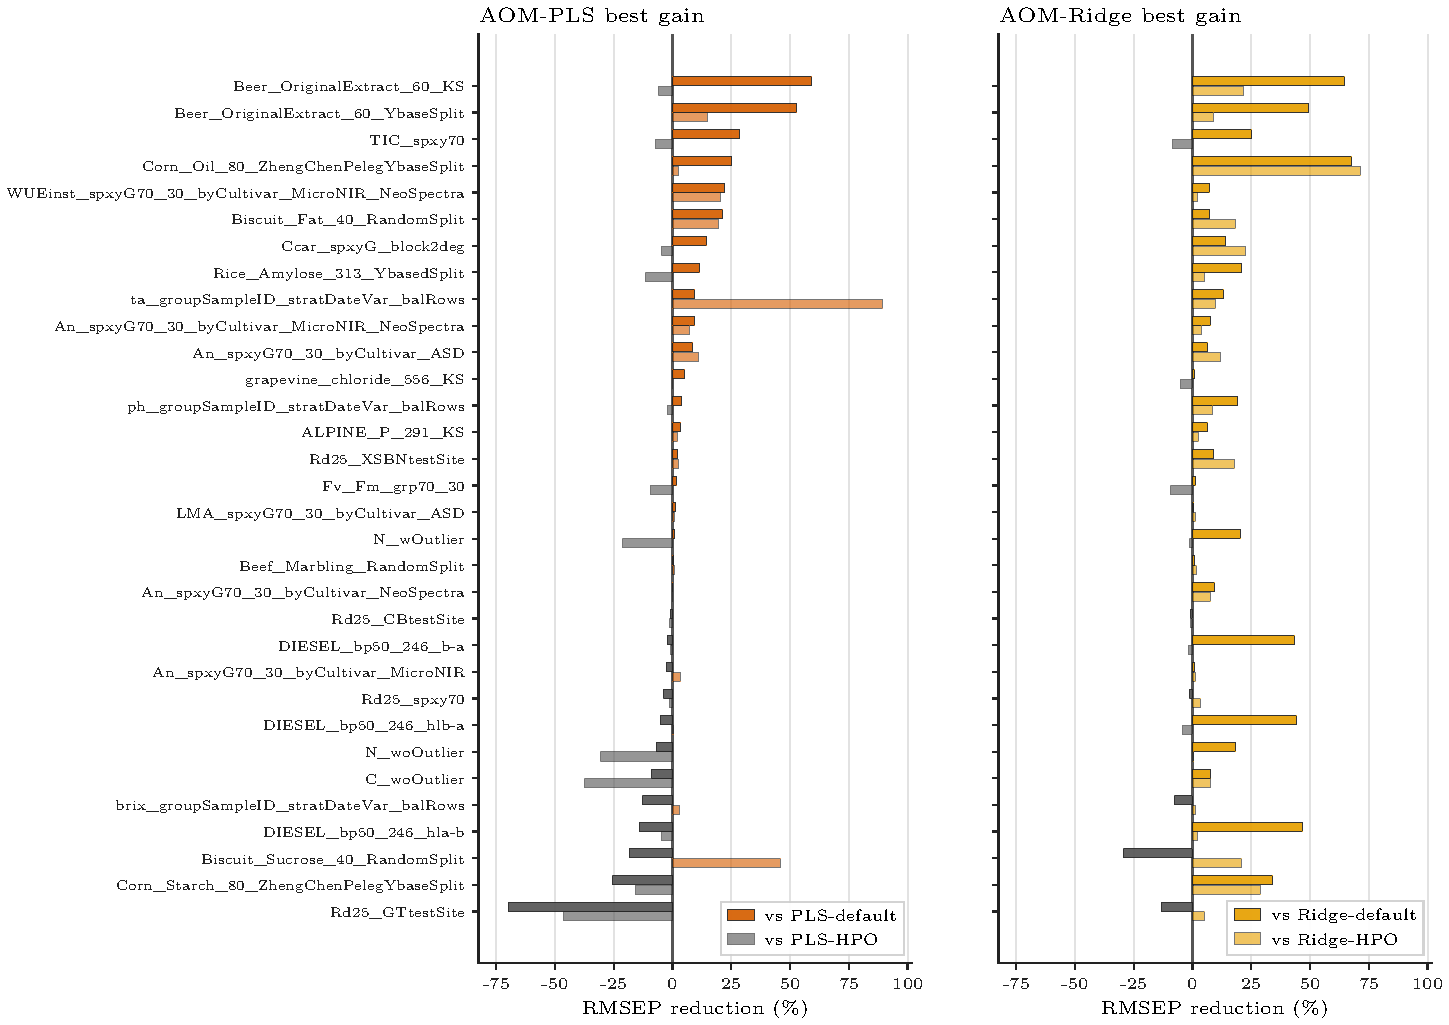
\includegraphics[width=\linewidth]{figures/fig_gain_per_dataset.pdf}
  \caption{Per-dataset RMSEP reduction for selected AOM variants.  Positive
  bars indicate lower RMSEP than the named reference; gray bars indicate a
  higher RMSEP.}
  \label{fig:sup_gain_per_dataset}
\end{figure}

\section{Classification Full Results}

\begin{table}[h]
\centering
\caption{Full classification paired comparisons.  Positive differences favour
the AOM or POP candidate over PLS-DA.}
\label{tab:sup_classification_full}
\small
\begin{tabularx}{\linewidth}{Xrrrr}
\toprule
Comparison & $N$ & Median $\Delta$ balanced acc. & 95\% CI & Wins; $p_{\mathrm{Holm}}$ \\
\midrule
AOM-\allowbreak{}PLS-\allowbreak{}DA-\allowbreak{}global-\allowbreak{}simpls-\allowbreak{}covariance vs PLS-\allowbreak{}DA & 13 & 0.159 & 0.129--0.422 & 12/13; 0.007 \\
POP-\allowbreak{}PLS-\allowbreak{}DA-\allowbreak{}simpls-\allowbreak{}covariance vs PLS-\allowbreak{}DA & 13 & 0.052 & 0.035--0.275 & 11/13; 0.018 \\
AOM-\allowbreak{}PLS-\allowbreak{}DA-\allowbreak{}global-\allowbreak{}nipals-\allowbreak{}adjoint vs PLS-\allowbreak{}DA & 13 & 0.030 & 0.000--0.111 & 8/13; 0.211 \\
POP-\allowbreak{}PLS-\allowbreak{}DA-\allowbreak{}nipals-\allowbreak{}adjoint vs PLS-\allowbreak{}DA & 13 & -0.037 & -0.098--0.048 & 5/13; 0.685 \\
AOMRidgeCls-\allowbreak{}global-\allowbreak{}compact vs PLS-\allowbreak{}DA & 14 & 0.175 & 0.145--0.264 & 13/14; 0.002 \\
AOMRidgeCls-\allowbreak{}branch\_\allowbreak{}global-\allowbreak{}compact vs PLS-\allowbreak{}DA & 14 & 0.169 & 0.137--0.272 & 13/14; 0.002 \\
AOMRidgeCls-\allowbreak{}superblock-\allowbreak{}compact vs PLS-\allowbreak{}DA & 14 & 0.165 & 0.124--0.243 & 14/14; 0.001 \\
AOMRidgeCls-\allowbreak{}active-\allowbreak{}compact vs PLS-\allowbreak{}DA & 14 & 0.163 & 0.118--0.228 & 14/14; 0.001 \\
AOMRidgeCls-\allowbreak{}mkl-\allowbreak{}compact vs PLS-\allowbreak{}DA & 14 & 0.163 & 0.129--0.234 & 13/14; 0.002 \\
\bottomrule
\end{tabularx}

\end{table}

The SIMPLS AOM-PLS-DA variant is the classification row promoted in the main
manuscript.  NIPALS-adjoint classifiers are less stable.  AOM-Ridge
classification variants are favourable on the 14-dataset overlap, but they
are kept here because the main classification question is the PLS-DA
covariance analogue.

\section{Seed Stability}

\begin{table}[h]
\centering
\caption{Seed-stability diagnostics for the multi-seed AOM-PLS and AOM-Ridge
runs.}
\label{tab:sup_seed_stability}
\small
\begin{tabularx}{\linewidth}{p{0.16\linewidth}Xrrrr}
\toprule
Family & Variant & Full seeds & Mean $\rho$ & Seed CV & Winner changes \\
\midrule
AOM-\allowbreak{}PLS & PLS-\allowbreak{}standard & 32 & 1.000 & 0.000 & 14 \\
AOM-\allowbreak{}PLS & AOM-\allowbreak{}compact-\allowbreak{}cv5 & 32 & 0.994 & 0.017 & 14 \\
AOM-\allowbreak{}PLS & ASLS-\allowbreak{}AOM-\allowbreak{}compact-\allowbreak{}cv5 & 32 & 0.994 & 0.021 & 14 \\
AOM-\allowbreak{}PLS & AOM-\allowbreak{}default & 32 & 1.000 & 0.000 & 14 \\
AOM-\allowbreak{}Ridge top5 & Ridge-\allowbreak{}raw & 23 & 1.000 & 0.000 & 0 \\
AOM-\allowbreak{}Ridge top5 & AOMRidge global compact & 23 & 1.000 & 0.000 & 0 \\
AOM-\allowbreak{}Ridge top5 & AOMRidge local knn50 & 23 & 1.000 & 0.000 & 0 \\
AOM-\allowbreak{}Ridge top5 & AOMRidge local blended & 23 & 1.000 & 0.000 & 0 \\
AOM-\allowbreak{}Ridge top5 & AOMRidge multibranch & 23 & 1.000 & 0.000 & 0 \\
\bottomrule
\end{tabularx}

\end{table}

AOM-PLS dataset-level RMSEP rankings are highly correlated across seeds, but
some datasets change the winning member of the AOM-PLS family.  The top AOM
Ridge rows are deterministic for the recorded split/random-state
representation.  FastAOM was run on seed0 for the wide exploration and
should be read as chain-space evidence rather than split-resampling evidence.

\section{Reproducibility and Software Artifacts}

\begin{table}[h]
\centering
\caption{Software artifacts distributed with the AOM study.}
\label{tab:sup_software}
\small
\begin{tabularx}{\linewidth}{p{0.30\linewidth} X p{0.20\linewidth}}
\toprule
Component & Tests / evidence & Status \\
\midrule
\texttt{nirs4all-aom} Python package & AOM-PLS, POP-PLS, AOM-Ridge and FastAOM implementations, with unit tests and sklearn-compatible APIs. & reference implementation \\
\texttt{nirs4all-methods} / \texttt{n4m} (C\texttt{++}) & Portable C\texttt{++} core with Python, R and JavaScript/WebAssembly entry points; matches the Python reference to numerical precision. & distributed implementation \\
\texttt{nirs4all-aom} benchmark artifacts & Benchmark runners, result CSVs, aggregation scripts, figure builders and manuscript tables used here. & versioned repository \\
\texttt{nirs4all} instrumentation context & NIRS instrumentation, acquisition and provenance context for local benchmark inputs. & instrumentation software \\
Supplementary validation dossier & Cohort manifest, missing-dataset audit, paired statistics and software-readiness notes distributed with \texttt{nirs4all-aom}. & public evidence \\
\bottomrule
\end{tabularx}

\end{table}

All numerical claims in the main manuscript and in this supplement are
computed from benchmark result tables distributed with the public
\code{nirs4all-aom} repository announced in the main manuscript.  The regression
cohort contains 61 manifest rows, and the main paired regression comparisons
use $N_{\cap}=32$ rows.  The classification manifest contains 17 rows, with 16
included in benchmark analyses after one missing-file exclusion, and is
summarized in the classification tables.

Multi-seed evidence is aggregated at dataset level before paired tests.
AOM-PLS, PLS-default, Ridge-default, PLS-HPO and Ridge-HPO use seeds 0, 1 and
2.  The AOM-Ridge headline selectors are reported on the deterministic
headline run with random state 0, while the supplementary seed-stability
table reports the multi-seed AOM-PLS and AOM-Ridge diagnostics.  The main
regression comparisons use paired dataset-level RMSEP ratios, Wilcoxon
signed-rank tests where applicable and Holm correction within the reported
comparison family.
Classification comparisons use paired balanced-accuracy differences with the
same family-wise correction.  The validation status of the software artifacts
is summarized in Table~\ref{tab:sup_software}.

\section{Declaration of Generative AI and AI-assisted technologies in the writing process}

During the preparation of this work, the authors used Anthropic Claude and
OpenAI Codex to assist with code review, implementation, repository
organization, benchmark aggregation scripts, LaTeX editing and drafting or
revision of explanatory text.  Every numerical claim in the main manuscript
and in this supplement is computed from benchmark result tables; the
AI-assisted tools did not generate numerical results by themselves.  After
using these tools, the authors reviewed, edited and verified the code,
numerical results, references and manuscript content as needed, and take full
responsibility for the content of the publication.

\nocite{geladi1986partial,wold2001pls,dejong1993simpls,hoerl1970ridge,rinnan2009review,savitzky1964smoothing,barnes1989standard,geladi1985linearization}

\bibliographystyle{unsrtnat}
\bibliography{references}

\end{document}
